\documentclass[11pt]{beamer}
\usepackage[utf8]{inputenc}
\usepackage[T1]{fontenc}
\usepackage{lmodern}
\usepackage{amsmath}
\usepackage{hyperref}
\usepackage{array}
\usepackage{amsfonts}
\usepackage{amssymb}
\usepackage{graphicx}
\usepackage{epstopdf}
\usepackage{caption}
\usepackage{multicol}
\usepackage{listings}
\usepackage{alltt}
\usepackage{mathtools}
\usepackage[makeroom]{cancel}
\usetheme{Frankfurt}
\usepackage{tikz} 
\usepackage{pgfplots}
\usetikzlibrary{patterns}
\usetikzlibrary{plotmarks}
\titlegraphic{\vspace{8cm}}% to push the other text to the top
\addtobeamertemplate{navigation symbols}{}{%
	\usebeamerfont{footline}%
	\usebeamercolor[fg]{footline}%
	\hspace{1em}%
	\insertframenumber/\inserttotalframenumber
	\setbeamercolor{footline}{fg=blue}
	\setbeamerfont{footline}{series=\bfseries}
}
\newcolumntype{M}[1]{>{\centering\arraybackslash}m{#1}}
		\newcommand\Fontvi{\fontsize{4}{7.2}\selectfont}
\begin{document}
	\author{\tiny
			L.F. Hiram Ernesto Dami\'an\\
			\vspace{5px}
				Director:\\
					\vspace{5px}
			Jos\'e Feliciano Ben\'itez Rubio\\
				\vspace{5px}
				Maestr\'ia en Ciencias (F\'isica)\\
					\vspace{5px}
			 Departamento de Investigacion en F\'isica }
	\title{Study of Higgs plus single top production using events with a same sign dimuon  at the Large Hadron Collider}
	%\subtitle{}
	\logo{
\includegraphics[scale=0.1]{unison-logo.png}}
	\newcommand{\nologo}{\setbeamertemplate{logo}{}}
	\institute{Universidad de Sonora}
	\date{\small November 25$^{th}$ 2019}
	%\subject{}
	\newcommand{\subf}[2]{%
		{\small\begin{tabular}[t]{@{}c@{}}
				#1\\#2
		\end{tabular}}%
	}
	%\setbeamercovered{transparent}
	%\setbeamertemplate{navigation symbols}{}
\begin{frame}
\titlepage
\end{frame}

\begin{frame}
\tiny
\tableofcontents
\end{frame}


%\begin{frame}
%\section{Overview and motivation}
%\frametitle{Overview}
%\begin{itemize}
%\item Through this project it was studied the production of Higgs boson in association with a
%single top quark ($tH$) in proton-proton collisions. 
%This mechanism of production of the Higgs boson has not been observed before by any
%experiment.
%\item Standard Model and the Higgs production mechanism
%\item A brief introduction to the LHC and CMS
%\item Event selection and reconstruction of the tH signal
%\item Creation and application of a statistical model for the analysis of events 
%\item Making predictions for the future experiments.
%\end{itemize}
%\end{frame}

\begin{frame}
\section{Introduction}
\subsection{Standard Model}
\frametitle{Standard Model}
\begin{table}
	\centering
\begin{tabular}{cc}
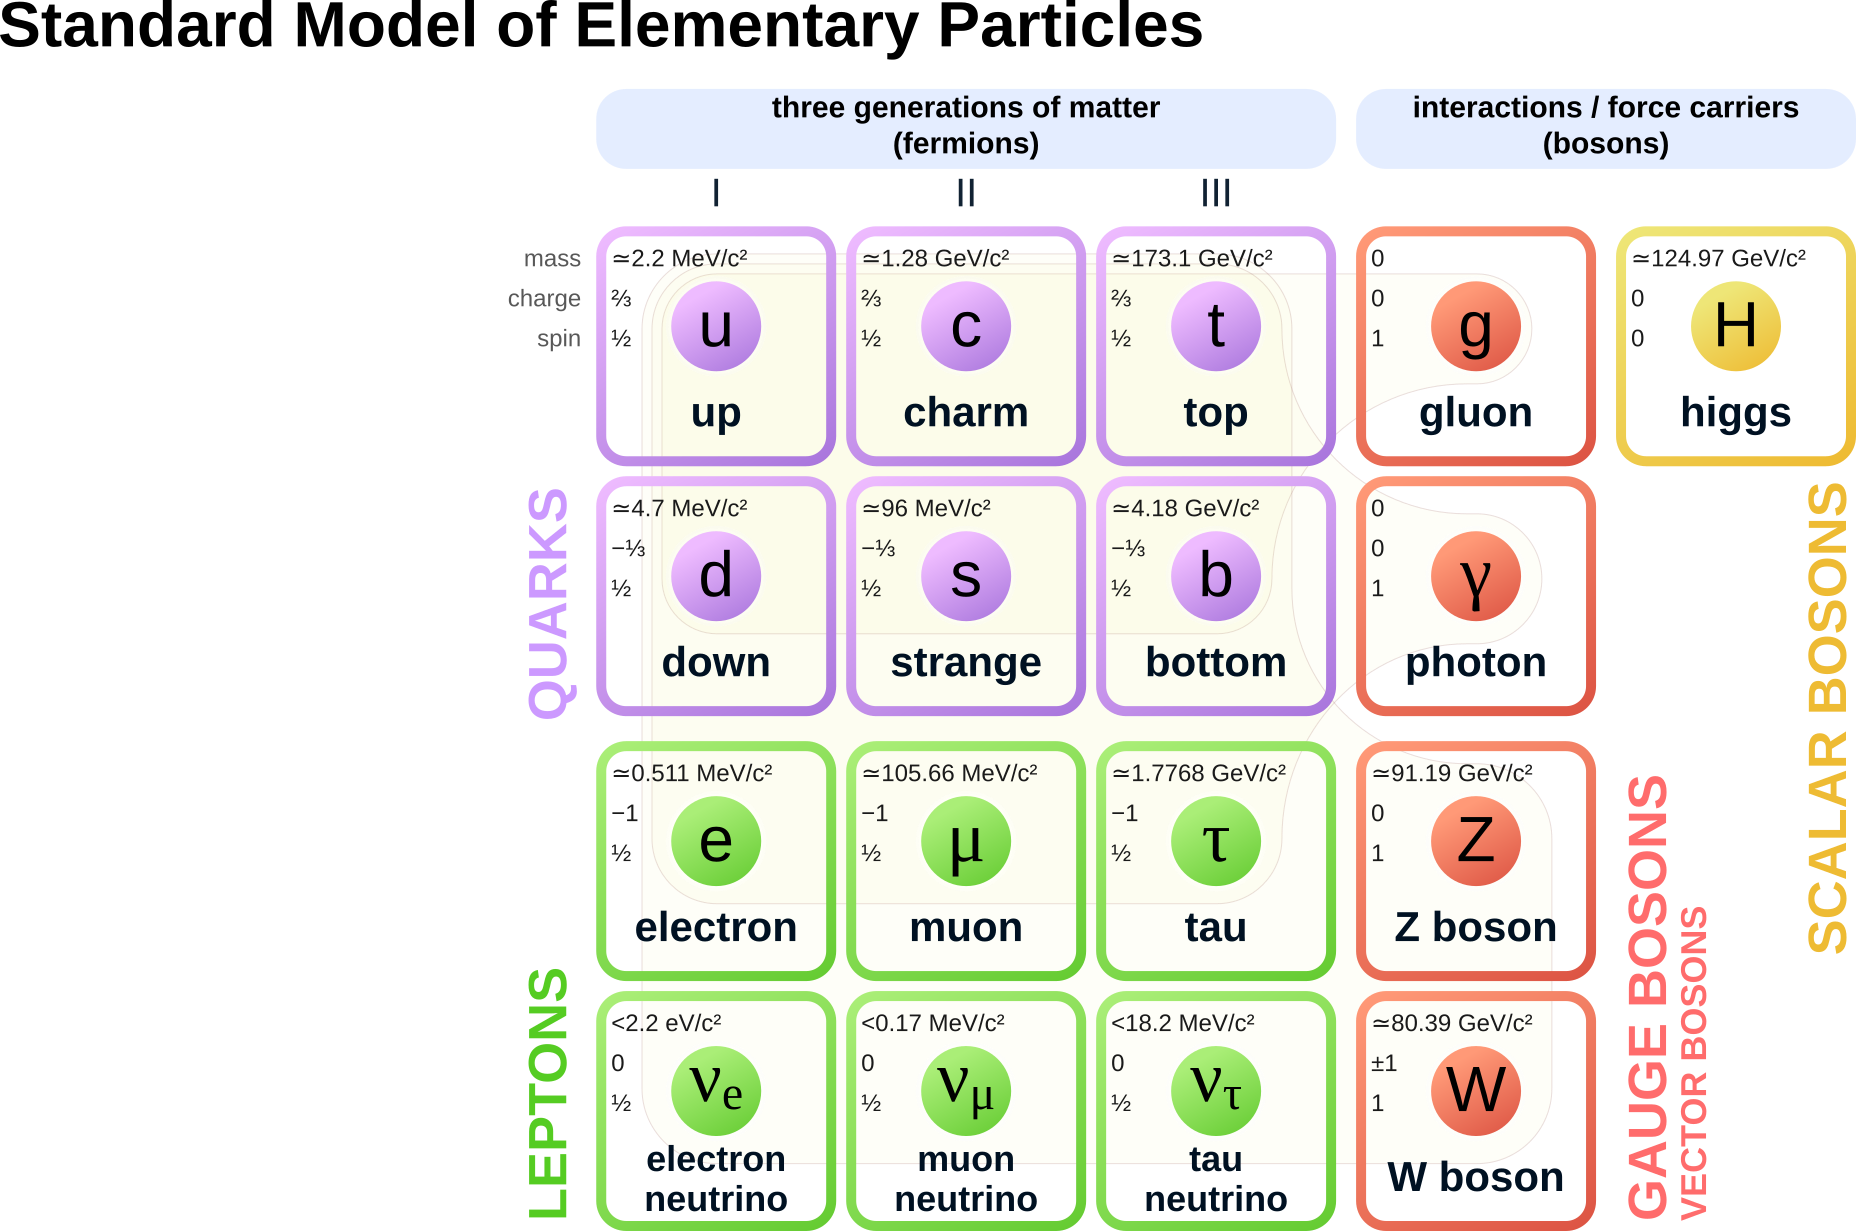
\includegraphics[width=6cm,height=5cm]{figures/sm1.png} & 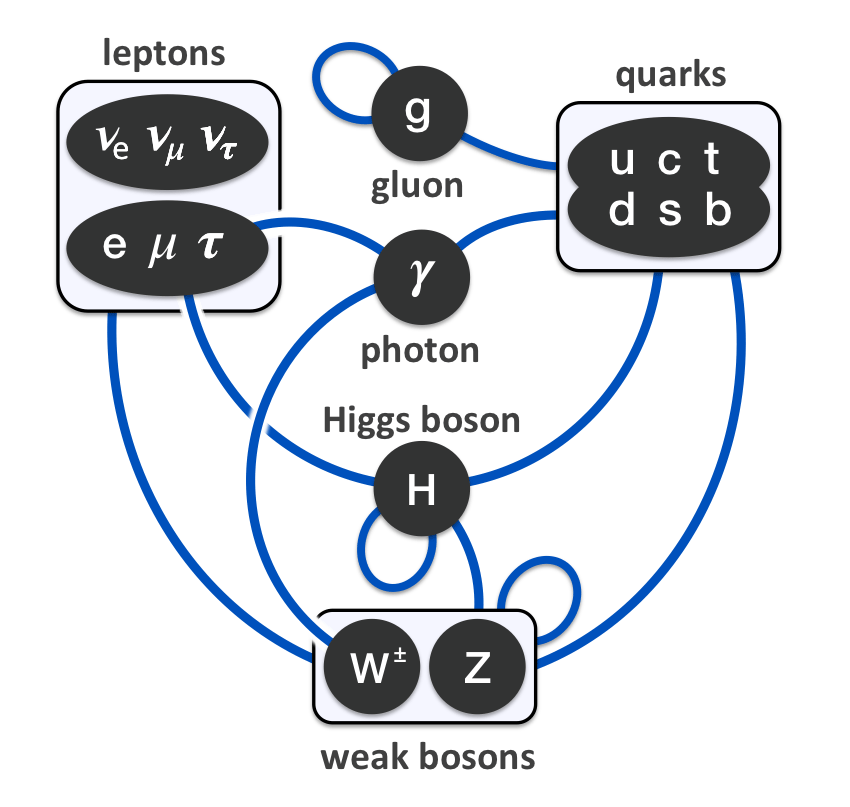
\includegraphics[width=5cm,height=5cm]{figures/sm.png}
\end{tabular}
\end{table}
\end{frame}

\begin{frame}
\frametitle{Motivation  for single top Higgs (tH)}
\begin{itemize}
\item Coupling measurement is essential to establish the nature of the Higgs
\item The exploration of Higgs production on the $tH$ channel is subject relatively new. Measurements of CMS and ATLAS are compatible with SM predictions.
\item The $tH$ study explores the relative sign of top-Higgs  and W-Higgs couplings.\\ Small deviations from SM predictions could be associated with physics beyond the
standard model (BSM) such as Supersymmetry.
\end{itemize}
\end{frame}

%\begin{frame}
%\subframetitle{Higgs mechanism}
%\frametitle{Electroweak SM Lagrangian}
%The Standard Model is a theory of fields for particles with spins 0, $\frac{1}{2}$ and 1. 
%The  SM lagrangian 	
%\begin{align*}
%\mathcal{L}=\mathcal{L}_\text{gauge}+\mathcal{L}_f +\mathcal{L}_\text{higgs} + \mathcal{L}_\text{yukawa}
%\end{align*}
%donde 
%\begin{itemize}
%	\item $\mathcal{L}_\text{gauge}$=$ -\frac{1}{4}\left[F^{\mu\nu}F_{\mu\nu}\right]-\frac{1}{4}\left[G^{i\mu\nu}G^i_{\mu\nu}\right]$ 
%	\begin{itemize}
%		\item  $F^{\mu \nu}=\partial_\mu B_\nu -\partial_\nu B_\mu $
%		\item  $G^{i\mu\nu}=\partial_\mu W^i_\nu -\partial_\nu W^i_\mu -g\epsilon^{ijk}W^j_\mu W^k_\nu $
%	\end{itemize}
%	\item $\mathcal{L}_f=i\bar{\Psi}_L \cancel{D}{\Psi}_L+i\bar{\psi}_R \cancel{D}{\psi}_R  $ is the kinematic term for fermions 
%\scriptsize{
%	\begin{itemize}
%		\item $D_\mu {\Psi}_L=\left(\partial_\mu+igW_\mu+ig'Y_LB_\mu\right)\Psi_L$
%		\item $D_\mu \psi_R=\left(\partial_\mu +ig' Y_RB_\mu\right)\psi_R $
%		\item g and g' are boson coupling constants.
%\footnote{\tiny{L(R) refers to Left and right fields.
%Y is the  weak hypercharge,Y=T$^3$-Q.Q is charge of particle field and T is weak isospin. $T^3=\pm 1/2$ for left handed doublets and $T^3=0$ for right handed singlets.} }
%\item $W_\mu=\sigma^iW^i_\mu$, where $\sigma^i$ are the pauli matrices.
%	\end{itemize}
%}
%\end{itemize}
%\begin{equation}
%\begin{split}
%\mathcal{L}=-\frac{1}{2}\text{Tr}\left[F^{\mu\nu}F_{\mu\nu} \right]+\bar{\Psi_L}i\gamma^\mu D_\mu \Psi_L  
%+\text{Tr}\left[(D_\mu \Phi)^\dagger (D^\mu \Phi)\right]+\mu^2 \Phi^\dagger \Phi  \\
%-\frac{1}{2}  \lambda (\Phi^\dagger \Phi)^2 & +\left(\frac{1}{2}\Psi_L^T Ch \Phi \Psi_L +h.c \right)
%\end{split}
%\end{equation}
%The matrix C in the last term is the charge conjugation matrix acting on the spinors, h is a matrix of Yukawa couplings
%\end{frame}

\begin{frame}
\subsection{Higgs mechanism}
\frametitle{Electroweak SM Lagrangian}
Higgs lagrangian 
\begin{align}
\mathcal{L}_{\text{Higgs}}=(D_\mu \Phi)^\dagger (D^\mu \Phi)-V(\Phi^\dagger \Phi)
\end{align}

with
\begin{itemize}
	\item $D_\mu \Phi = \left(\partial_\mu+(ig/2)\sigma^iW^i_\mu-i\frac{1}{2} g' B_\mu \right) \Phi $
	\item $V(\Phi^\dagger \Phi)=-\mu^2 \Phi^\dagger \Phi +\frac{1}{2}  \lambda (\Phi^\dagger \Phi)^2, \quad \mu^2>0  $ 
	\item $\Phi=\left(\begin{array}{c}
	\phi^+ \\
	\phi^0
	\end{array} \right)  $ is a SU(2) doublet.
	\item $\sigma^i$ are the Pauli matrices.
\end{itemize}
 
\begin{itemize}
	\item $\Phi$ is Higgs field which is a complex scalar field. $\Phi$
	%\item  W$_\mu$ and B$_\mu$ are gauge bosons
	%\item g and g are boson coupling constants.
	\item $\lambda $ and $\mu^2$ are Higgs potential parameters
\end{itemize}
\end{frame}

\begin{frame}
\frametitle{Electroweak SM Lagrangian}
	\begin{figure}[ht!]
		\centering
		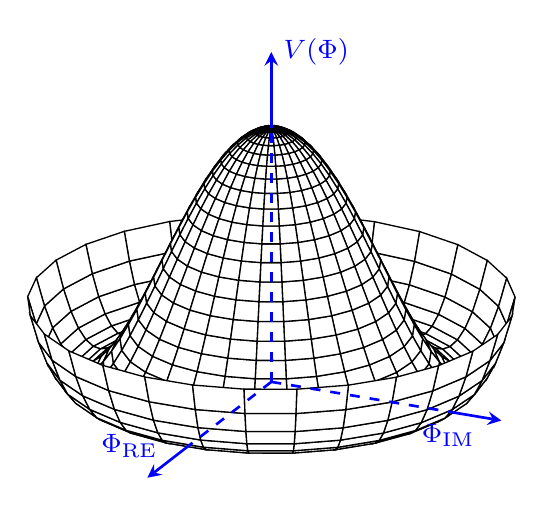
\begin{tikzpicture}[scale=1.2]
		\begin{axis}[
		hide axis,
		%axis lines=middle,
		%      axis on top,
		%      axis line style={blue,dashed,thick},
		%      ymin=-2,ymax=2,
		%      xmin=-2,xmax=2,
		%      zmin=-2,zmax=2,
		samples=30,
		domain=0:360,
		y domain=0:1.25,clip=false
		]
		\addplot3 [surf, shader=flat, draw=black, fill=white, z buffer=sort]
		({sin(x)*y}, {cos(x)*y}, {(y^2-1)^2});
		\draw[blue,thick,dashed] (axis cs:0,0,0) -- (axis cs:1,0,0)
		node[below,font=\footnotesize]{$\Phi_{\text{IM}}$};
		\draw[blue,thick,-stealth] (axis cs:1,0,0) -- (axis cs:1.3,0,0)
		node[above,font=\footnotesize]{};
		\draw[blue,thick,dashed] (axis cs:0,0,0) -- (axis cs:0,-1,0)
		node[left=2mm,font=\footnotesize]{$\Phi_{\text{RE}}$};
		\draw[blue,thick,-stealth] (axis cs:0,-1,0) -- (axis cs:0,-1.5,0)
		node[right=1mm,font=\footnotesize]{};
		\draw[blue,thick,dashed] (axis cs:0,0,0) -- (axis cs:0,0,1)
		%node[left=2mm,font=\footnotesize]{$\phi_{\text{RE}}$}
		;
		\draw[blue,thick,-stealth] (axis cs:0,0,1) -- (axis cs:0,0,1.3)
		node[right,font=\footnotesize]{$V(\Phi)$};
		\end{axis}
		\end{tikzpicture}
		\caption*{\small Higgs potential $V(\Phi^\dagger \Phi)$ for $\mu^2<0$ and $\lambda>0$, also called the mexican hat potential.}
		\label{hat}
	\end{figure}
\end{frame}
\begin{frame}
\frametitle{SM Lagrangian}
Yukawa lagrangian
\begin{align}
\mathcal{L}_\text{yukawa}=\sum_{m,n}^{3}  \Gamma^u_{mn}\bar{q}_{m\text{,}L} \tilde{\Phi} u_{n\text{,}R}%+\Gamma^d_{mn}\bar{q}_{m\text{,}L} \Phi d_{n\text{,}R}+\Gamma^e_{mn}\bar{l}_{m\text{,}L} \Phi e_{n\text{,}R}+h.c
\end{align}
\scriptsize{where h.c is hermitian conjugate. m and n are flavors of quarks and leptons.
\\
The matrices $\Gamma_{mn}$ describe the so called Yukawa couplings between higgs doublet $\phi$ and the fermions.\\
Choosing}
\begin{align*}
\Phi=-\frac{1}{2}\left(\begin{array}{c}
0 \\
v+h
\end{array} \right) \label{vmin}
\end{align*}
\scriptsize{
By using \ref{vmin} it on $\mathcal{L}_\text{yukawa}$, it is obtained for $u$ quark
\begin{align*}
\frac{\Gamma^u_{uu}v}{\sqrt{2}}(\bar{u_L}u_R+\bar{u_R}u_L)
\end{align*}
from which the masses for the fermions shown to be proportional to the Yukawa couplings
\begin{align*}
m_u=-\frac{\Gamma^u_{uu}v}{\sqrt{2}}
\end{align*}}
\end{frame}

\begin{frame}
\frametitle{Particles Properties}
Table of particles in SM
\begin{table}
\tiny{\renewcommand{\arraystretch}{1.5}
\begin{tabular}{|c|c|c|c|c|p{2.5cm}|}
\hline 	
Particle	& Mass (MeV/$c^2$) &Charge & spin &Lifetime (s) & Distance in lifetime (meters) \\ 
\hline 
Up ($u$)	& 2.2 & $\frac{2}{3}$ & $\frac{1}{2}$ & stable & -\\ 
\hline 	
Charm ($c$)	& 1280 &$\frac{2}{3}$ & $\frac{1}{2}$ & $ 1.1 \times 10^{-12}$ & 5.21$\times 10^{-3}$ \\ 
\hline 
Top	($t$)& 173100 & $\frac{2}{3}$ & $\frac{1}{2}$ & 5$\times$10$^{-25}$ &2.37$\times 10^{-15}$  \\ 
\hline 
Down ($d$)	& 4.6 &$-\frac{1}{3}$ & $\frac{1}{2}$ & Stable & - \\ 
\hline 
Strange ($s$)	& 96 &$-\frac{1}{3}$ & $\frac{1}{2}$ &$1.24 \times 10^{-8}$ & 58.7 \\ 
\hline 
Bottom ($b$)	& 4180 &$-\frac{1}{3}$ & $\frac{1}{2}$ &$1.3 \times 10^{-12}$  & 6.16 $\times 10^{-3}$\\ 
\hline 
$W$ 	& 80379 &$\pm$1 & 1 & 3$\times$ 10$^{-25}$ & 1.42$\times 10^{-15}$\\ 
\hline 
$Z$ & 91187.6 &0 & 1 & 3$\times$ 10$^{-25}$ &1.42$\times 10^{-15}$ \\ 
\hline
Photon ($\gamma$) & 0 &0 & 1&Stable & - \\ 
\hline
Gluon ($g$)	& 0 &0 & 1&Stable & - \\ 
\hline 
Higgs ($H$)	& 125.18 &0 & 0& 1.56 $\times$ $10^{-22}$ & 7.39$\times 10^{-13}$ \\ 
\hline 
Electron ($e$)& 0.511 & -1 &  $\frac{1}{2}$& Stable & - \\ 
\hline 
Muon ($\mu$)	& 105.7 & -1 & $\frac{1}{2}$ & 2.2$\times$10$^{-6}$ & 10419.85 \\ 
\hline 
$\tau$	& 1776.86 &-1 & $\frac{1}{2}$ & 2.9$\times$10$^{-13}$ & 1.37$\times 10^{-3}$\\ 	
\hline 
$\nu_e$	$\nu_\mu$ $\nu_\tau$& 0 & 0 & $\frac{1}{2}$ & Stable & -\\
\hline 
\end{tabular} 
}
\end{table}
\tiny{Stable means no decay, or lifetime almost infinite. Particles speeds at $v$=0.998c}
\end{frame}

{\nologo
\begin{frame}
\subsection{Higgs production mechanisms and decays}
\frametitle{Higgs production mechanisms}

\begin{center}
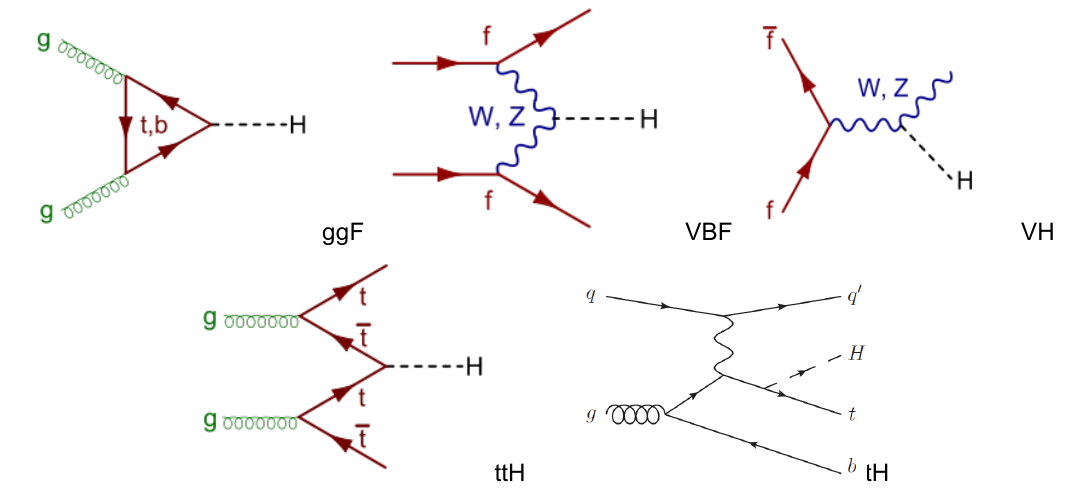
\includegraphics[scale=0.4]{figures/pg.png}
\end{center}
\small{Different Higgs production mechanism, from the most likely to least likely}
\end{frame}
}

\begin{frame}
\frametitle{Cross section}
\begin{itemize}
\item Cross section describes the likelihood of two particles interacting under certain conditions\cite{1}\cite{6}
\begin{align}
N_R=\sigma \text{L}
\end{align}
%\item Experimentally
%\begin{align}
%d\sigma=\frac{\text{number of particles scattered into solid angle} \Delta\Omega}{\text{(number of particles incident)(scattering centers/area)}}
%\end{align}
\item Cross sections are expressed in barns , where 1 barn=$10^{-34}$ cm$^{-2}$ 
\item The reaction rate $N_R$ is determined by the total cross section $\sigma$ and the incident flux L.\\
L is called luminosity and it is measured in cm$^{-1}$s$^{-1}$.\cite{6}
\end{itemize}
\end{frame}

\begin{frame}
\frametitle{Higgs production Cross section}
\begin{table}
	\caption*{Higgs boson production cross sections  in pp collisions for $\sqrt{s}=13$TeV  (in
		pico barn).Integrated luminosity of 35.9 fb$^{-1}$ for Run 2\footnotemark}
	\begin{tabular}{|c|c|c|}
		\hline
		Production mechanism &
		$\sigma$ (picobarns pb)
		&Number of events \\
		\hline
		ggF &
		48.93 &
		1756587\\
		\hline
		VBF &
		3.78&
		135702\\
		\hline
		WH & 1.35 & 48465\\
		\hline
		ZH &0.88 & 31592\\
		\hline
		t$\bar{t}$H &
		0.50&
		18255\\
		\hline
		$tH$ &
		0.015&
		560.39\\
		\hline
	\end{tabular}
\end{table}

\footnotetext[1]{\tiny{Data taken from The cern collaborarion “Higgs Physics the HL-LHC and HE-LHC” 2019, CERN-LPCC-2018-04}}

\end{frame}



\begin{frame}
\frametitle{Branching ratio}
\small{In particle physics, the branching ratio for a decay process is the ratio of the number of particles which decay via a specific decay mode with respect to the total number of particles which decay via all decay modes. \footnotemark.}
\begin{align}
\text{BR} =\frac{\Gamma_i}{\sum_{i}\Gamma_i}
\end{align}
\small{Where $\Gamma=\sum_i\Gamma_i$ is the total decay width (sum of all partial widths) of the particle and is related to lifetime of the particle: $\Gamma=1/\tau$.
Since the dimension of $\Gamma$ is the inverse of time, in our system of natural units, it is measured in inverse seconds} .%it has the same dimension as mass (or energy).}
\footnote[0]{\tiny{Cleaves H.J. (2011) Branching Ratio. In: Gargaud M. et al. (eds) Encyclopedia of Astrobiology. Springer, Berlin, Heidelberg} }
\end{frame}
 


\begin{frame}
\frametitle{Higgs Branching ratios per channel}
\begin{table}
	\caption*{SM Higgs boson branching ratios for  $M_H$ =125 GeV}
\begin{center}
\begin{tabular}{|c|c|}
	\hline
	Higgs decay & Branching ratio (BR)\\
	\hline
	H $\rightarrow$ b$\bar{b}$ &
	$50.82\%$ \\
	\hline
	H $\rightarrow$ $W^+W^-$ &
	$21.5\%$ \\
	\hline
	H $\rightarrow$ $\tau^+ \tau^-$ &
	$6.27\%$\\
\hline
	H $\rightarrow$ ZZ &
$2.61\%$\\
\hline
	H $\rightarrow$ $\gamma\gamma$ &
$0.227\%$\\
\hline
	H $\rightarrow$ Z$\gamma$ &
$0.153\%$\\
\hline
	H $\rightarrow$ $\mu^+\mu^-$ &
$0.0217\%$\\
\hline
\end{tabular}
\end{center}
\end{table}

\end{frame}

{\nologo
\begin{frame}
\frametitle{$tH$ production mechanisms}
\begin{center}
\begin{figure} 
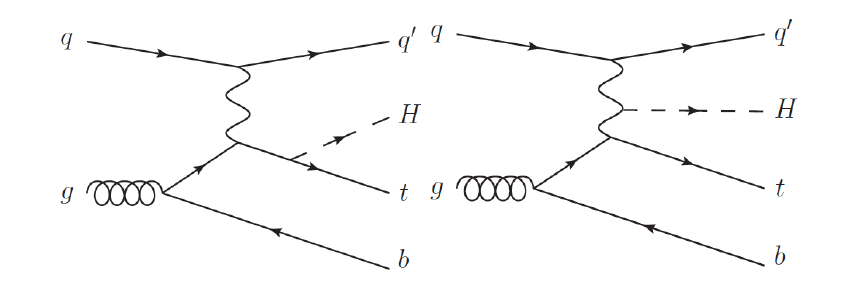
\includegraphics[scale=0.4]{figures/tq.png} 
\caption*{$tH$ mechanism. Higgs radiated from a top quark (left). Higgs radiated from a W boson (right)} 
\label{th}
\end{figure}
\end{center}
\end{frame} 
}

\begin{frame}
\frametitle{$tH$ production mechanisms}
\begin{itemize}
\item In a proton proton collision, the production cross section of the single top plus Higgs boson process is driven by a
destructive interference of two main diagrams, where the Higgs couples to either
the W boson or the top quark. 
\item  A second process, where the Higgs and top quark
are accompanied by a W boson ($tH$W) has similar behavior, albeit with a weaker interference
pattern.
\item However, in the presence of new physics, there may be relative opposite signs between the $tH$
and WH couplings which lead to constructive interference and enhance the cross sections by
an order of magnitude or more.
\end{itemize}
\end{frame}

\begin{frame}
\frametitle{$\mu\mu$ same sign decay rate}
\tiny{Table of decay chains for tH.  Expected number of $tH$ final states events for 35.9 fb$^{-1}$.l represents $\mu^{\pm},e^- , \tau^\pm$. }
\begin{table}
\renewcommand{\arraystretch}{0.55}
\begin{tabular}{|p{8cm}|p{1.3cm}|c|}
\hline
Decay chain &BR&Events\\
\hline 
\tiny{$tH \rightarrow$ W$^+$bW$^+$W$^-$ $\rightarrow$ $\mu^+$ $\nu_\mu$b$\mu^+\nu_\mu$  $q \bar{q}'$ } &\tiny{2.096 $\times$10$^{-3}$} &  1.173  \\
\hline
\tiny{$tH \rightarrow $W$^+$bW$^+$W$^-$ $\rightarrow$ $\mu^+\nu_\mu$b$\mu^+\nu_\mu$ $l^- \bar{\nu_l}$ } &\tiny{3.37 $\times$ 10$^{-4}$} &0.899 \\
\hline
\tiny{$tH \rightarrow$ W$^+$b $\tau^+ \tau^-$ $\rightarrow$ $\mu^+ \nu_\mu$ b $ \mu^+ \nu_\mu \bar{\nu_\tau} l^-\bar{\nu_l} \nu_\tau$} &\tiny{3.637$\times$10$^{-4}$}&0.203 \\
\hline
\tiny{$tH \rightarrow$ W$^+$bW$^+$W$^-$ $\rightarrow$ $\tau^+ \bar{\nu_\tau}$b $\mu^+ \nu_\mu$  $q\bar{q}$ $\rightarrow$ $\mu^+ \nu_\mu$ $\bar{\nu_\tau}$ $\bar{\nu_\tau}$ b$\mu^+ \nu_\mu$  $q \bar{q}$} &\tiny{1.890$\times$10$^{-4}$}&0.105  \\
\hline
\tiny{$tH \rightarrow$ W$^+$b $\tau^+ \tau^-$ $\rightarrow$ $\mu^+$ $\nu_\mu$b $\nu_\tau$ $\mu^+$ $\nu_\mu \bar{\nu_\tau}$} $q \bar{q}$  &
\tiny{1.681 $\times$10$^{-4}$} & 0.094 \\
\hline
\tiny{$tH \rightarrow$ W$^+$b W$^+$W$^-$ $\rightarrow$ $\tau^+ \bar{\nu_\tau}$b$ \mu^+ \nu_\mu l^- \bar{\nu_l}$ $\rightarrow$ $\mu^+\nu_\mu$ $ \bar{\nu_\tau} \bar{\nu_\tau}$  b$ \mu^+ \nu_\mu l^- \bar{\nu_l}$} &\tiny{3.045$\times$10$^{-5}$}& 0.017\\
\hline
\tiny{$tH \rightarrow$ W$^+$bZZ $\rightarrow$ $q \bar{q}$bZZ $\rightarrow$ $q \bar{q} $ b $\mu^+ \mu^- \mu^+ \mu^-$} & \tiny{1.966$\times$10$^{-5}$} &0.011\\
\hline 
\tiny{$tH \rightarrow$ W$^+$b $\tau^+ \tau^-$ $\rightarrow$ $\tau^+ \bar{\nu_\tau}b$ $\mu^+ \nu_\mu \bar{\nu_\tau} $  $q\bar{q}' \nu_\tau$ $\rightarrow$  $\mu^+ \nu_\mu \bar{\nu_\tau}\bar{\nu_\tau} $b $\mu^+ \nu_\mu \bar{\nu_\tau} $  $q\bar{q}' \nu_\tau$ } &\tiny{1.549 $\times$10$^{-5}$} &  0.008  \\
\hline
%\tiny{$tH \rightarrow$W$^+$bZ$\gamma$ $\rightarrow$ $\mu^+ \nu_\mu$ b $\mu^+ \mu^- \gamma$} & \tiny{6.888$\times$10$^{-6}$}&0.003\\
%\hline 
%\tiny{$tH \rightarrow$W$^+$bZZ $\rightarrow$ $\mu^+ \nu_\mu$ b $\mu^+ \mu^- l^+l^-$} &\tiny{3.962$\times$10$^{-6}$ }&0.002\\
%\hline 
%%\tiny{$tH \rightarrow$ $\tau \nu_\tau $bZ$\gamma$ $\rightarrow$ $\mu^- \bar{\nu_\mu} \nu_\tau \nu_\tau$ b $\mu^+ \mu^- \gamma$} & 6.347$\times$10$^{-7}$ & 0.0003\\
%%\hline 
\end{tabular}
\end{table}
\end{frame}

\begin{frame}
\section{LHC and CMS}
\subsection{LHC}
\frametitle{LHC}
	\begin{figure}
		\centering
	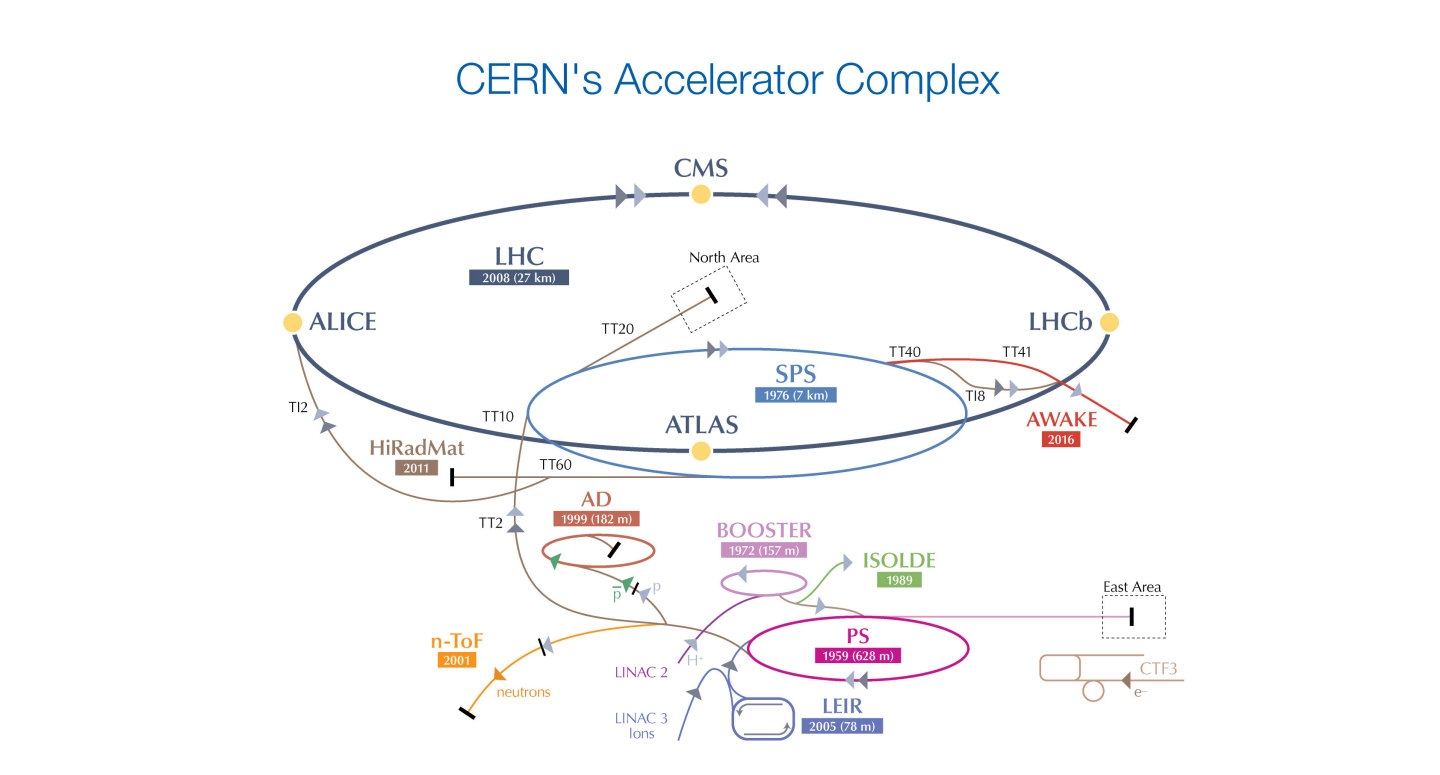
\includegraphics[scale=0.2]{figures/CERN's-accelerator-complex2013.jpg}
	\caption*{LHC complex}
	\end{figure}
\end{frame}

\begin{frame}
\frametitle{LHC}
\begin{figure}
	\centering
	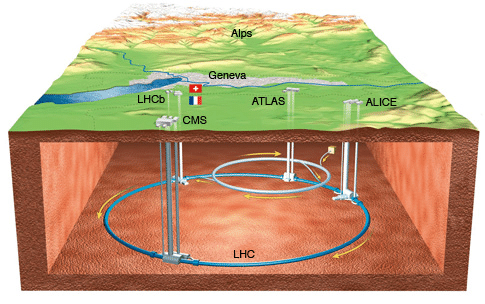
\includegraphics[scale=0.6]{figures/lhc-u.png}
	\caption*{Underground view of LHC complex}
\end{figure}
\end{frame}

\begin{frame}
\frametitle{LHC parameters}
\begin{minipage}[c]{0.48\textwidth}
	\tiny
\begin{table}
	\caption*{Characteristics of LHC}
\centering
\begin{tabular}{|c|c|}
			\hline
			Quantity & Number \\
			\hline
			Circumference &  26 659 m \\
			\hline
			Number of magnets& 9593 \\
			\hline
			Nominal energy, protons & 6.5 TeV\\
			\hline
			Nominal energy, protons collisions &  13 TeV\\
			\hline
			Number of collisions per second &1 billion\\
			\hline
			No. of bunches per proton beam &  2808\\
			\hline
\end{tabular}
\end{table}
\end{minipage}
\hfill
\begin{minipage}[c]{0.48\textwidth}
	\tiny
	\begin{table}
		\centering
		\caption*{Accelerator operation energies}
		\begin{tabular}{|c|c|}
			\hline
			Accelerator & Energy \\
			\hline
			Linac 2 &  50 MeV \\
			\hline
			PS Booster & 1.4 GeV \\
			\hline
			Proton Scyncroton (PS) & 25 GeV\\
			\hline
			SPS &  450 GeV\\
			\hline
			LHC & 6.5 TeV\\
			\hline
		\end{tabular}
	\end{table}
\end{minipage}
\end{frame}

\begin{frame}
\subsection{CMS dectector}
\frametitle{CMS detector}
\begin{center}
	\begin{figure}
		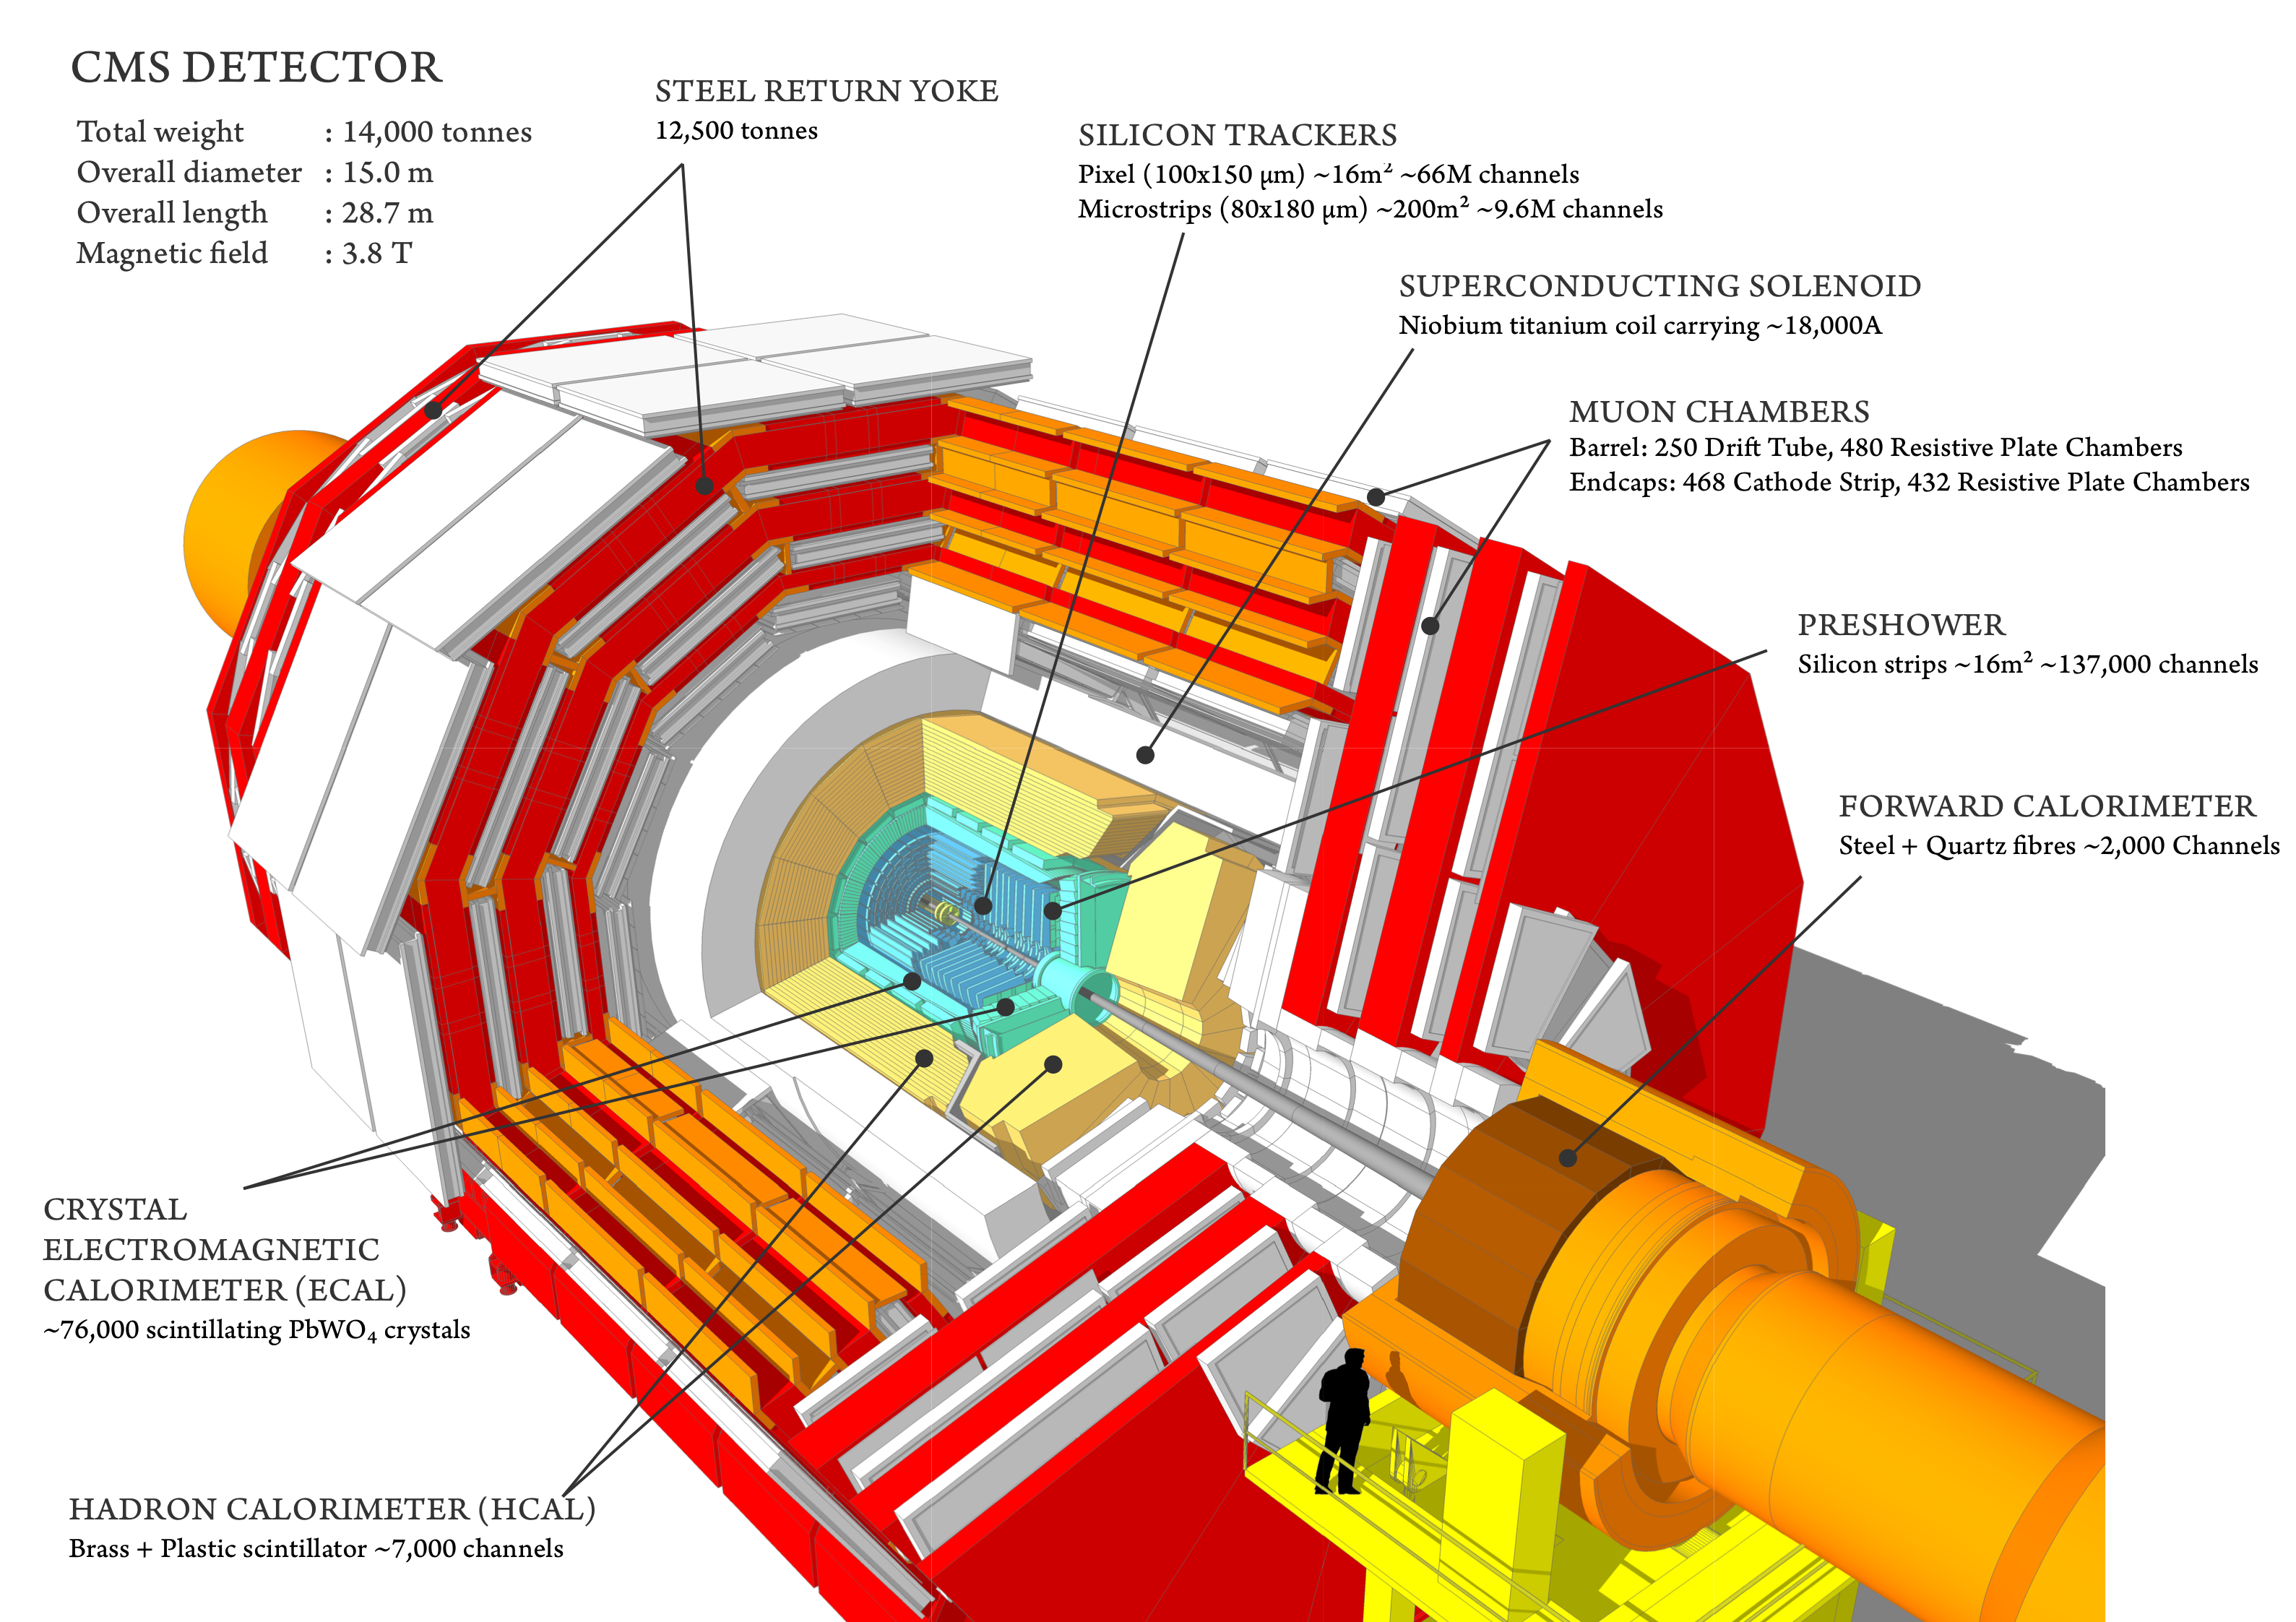
\includegraphics[scale=0.08]{figures/cms.png}
		\caption*{Compact muon solenoid}
	\end{figure}
\end{center}
\end{frame}


\begin{frame}
\frametitle{CMS detector}
\begin{figure}[ht!]
	\centering
	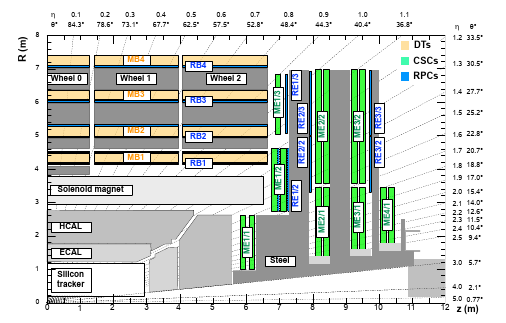
\includegraphics[scale=0.6]{figures/csc.png}
	\caption*{Slide view of the CMS in terms of pseudorapidity $\eta=-\ln\left[\tan\left(\frac{\theta}{2}\right)\right]$}
\end{figure}
\end{frame}

\begin{frame}
\frametitle{CMS detector}
\begin{figure}
	\centering
	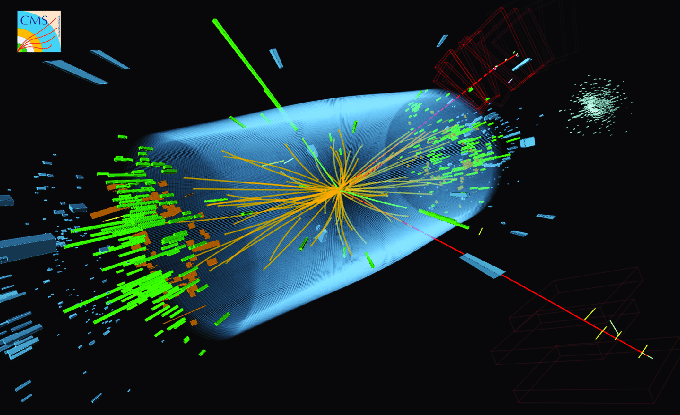
\includegraphics[scale=0.4]{figures/pp.png}
	\caption*{\small A typical CMS event display of the Higgs boson decaying to four leptons with 2 muons (in red) and 2 electrons (in green) as final state signatures.}
\end{figure}
\end{frame}

\begin{frame}
\frametitle{CMS integrated luminosity}
\begin{center}
	\begin{figure}
		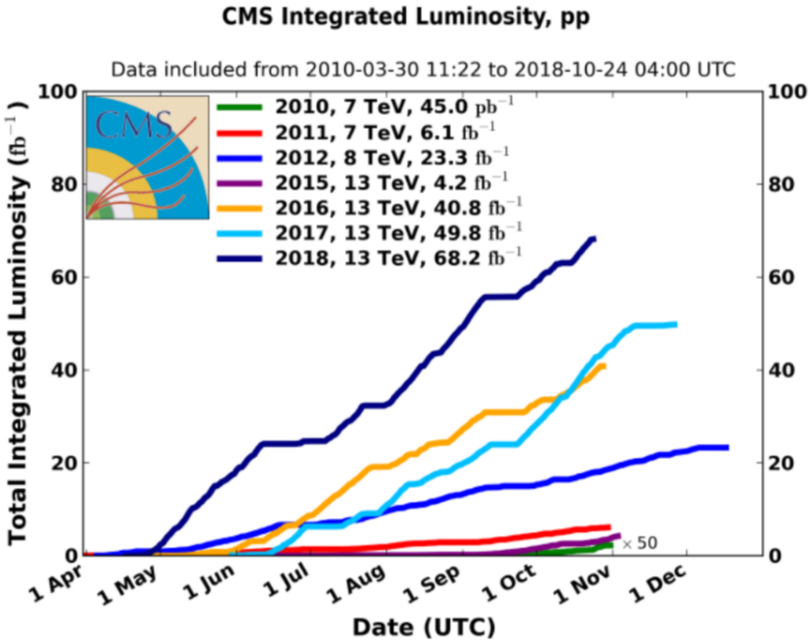
\includegraphics[scale=0.3]{figures/cms_lumi.png}
		\caption*{Integrated luminosity for CMS experiment }
	\end{figure}
\end{center}
\end{frame}




\begin{frame}
\section{Event selection and reconstruction}
\subsection{Topology of $tH$}
\frametitle{Topology of events tH}
The characteristics of the signal $tH$:

\begin{multicols}{2}
	\small{
\begin{itemize}
\item $t\rightarrow W$$^+$b$\rightarrow$ $l^+ \nu_\mu b$
\item $H\rightarrow$ $W^+$$W^-$ 

\begin{list}{--}{}
\item  \small{$W\rightarrow$ $l^\pm \nu$, where $l$ can be $\mu^\pm$,$e^-$  $\tau^\pm$} 
\item   \small{$W\rightarrow$ $q\bar{q}$}
\item \small{$W$ bosons decay leptonically resulting in a signature of two same-sign leptons }
\end{list}
\item a light-flavor quark 
\item  A b-jet  
\end{itemize}
}
\columnbreak
\begin{figure}
	\centering
	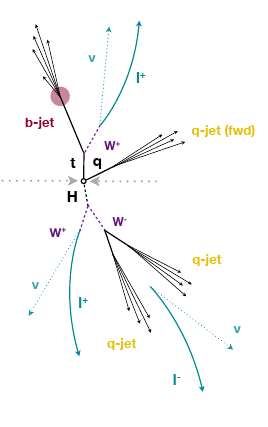
\includegraphics[scale=0.5]{figures/jet.png}
\end{figure}
\end{multicols}
\end{frame}

%\begin{frame}
%\frametitle{Backgrounds}
%\subsection{Backgrounds}
%\begin{itemize}
%	\item Backgrounds are considered information in the data that is not the signal. 
%	\item Backgrounds share certain characteristics of the signal.
%	\item Backgrounds are a big factor in the statistical study of the signal.
%\end{itemize}
%\end{frame}

\begin{frame}\subsection{Main backgrounds}
\frametitle{Main backgrounds}
\tiny
\begin{table}
	\caption*{Main backgrounds and their same sign $\mu\mu$ decay process }
	\centering
	\begin{tabular}{|c|l|}
		\hline
		Background & Decay process \\
		\hline
		$t\bar{t}W$ &$t\bar{t}W$ $\rightarrow$ $W^+ b W^- \bar{b}$ $\mu^+\nu_\mu$ $\rightarrow$ $\mu^+ \nu_\mu b$ $\mu^- \bar{\nu_\mu} \bar{b}$ $\mu^+ \nu_\mu$\\
		\hline
		$t\bar{t} Z$ & $t\bar{t} Z$ $\rightarrow$ $W^+ b$ $W^-\bar{b} \mu^+ \mu^-$ $\rightarrow$ $\mu^+ \nu_\mu b$ $\mu^- \bar{\nu_\mu} \bar{b}\mu^+ \mu^-$ \\
		\hline
		$W^+ Z$ &$W^+ Z \rightarrow$ $\mu^+ \nu_\mu \mu^+ \mu^-$ \\
		\hline 
		$W^\pm$ $W^\pm$ & $W^+W^+$ $\rightarrow$$\mu^+\nu_\mu$$\mu^+ {\nu_\mu}$ \\
		\hline 
		$tZq$ & $tZq$ $\rightarrow$ $W^+$ $ b\mu^+ \mu^- q$ $\rightarrow$$\mu^+ \nu_\mu b$ $\mu^+\mu^- q$ \\
		\hline 
		$t\bar{t}t\bar{t}$ &$t\bar{t}t\bar{t}$ $\rightarrow$ $W^+ b$ $W^- \bar{b}$ $W^+ b$ $W^- \bar{b}$ $\rightarrow$ $\mu^+ \nu_\mu b$ $\mu^- \bar{\nu_\mu} \bar{b}$ $\mu^+ \nu_\mu b$ $\mu^- \bar{\nu_\mu} \bar{b}$ \\
		\hline 
		$W^+ W^- Z$ & $W^+ W^-$ $Z \rightarrow$ $\mu^+ \nu_\mu$ $\mu^- \bar{\nu_\mu} \mu^+ \mu^-$\\
		\hline 
		$ZZZ$ & $ZZZ \rightarrow$ $\mu^+ \mu^-\mu^+ \mu^-l^+ l^-$ \\
		\hline 
		$W^+ZZ$ &$W^+ZZ$ $\rightarrow$ $\mu^+ \nu_\mu \mu^+ \mu^- l^+l^-$ \\
		\hline 
		$tZW^+$ & $tZW^+ \rightarrow$ $W^+b \mu^+ \mu^- \mu^+ \nu_\mu \rightarrow \mu^+ \nu_\mu b \mu^+ \mu^- \mu^+ \nu_\mu$\\
		\hline
		$ZZ$ & $ZZ\rightarrow$ $\mu^+ \mu^- \mu^+ \mu^-$ \\
		\hline
		$t\bar{t}H$	& $t\bar{t}H$ $\rightarrow W^+b W^- \bar{b} W^+W^-$ $\rightarrow$ $\mu^+ \nu_\mu b$$\mu^- \bar{\nu_\mu}\bar{b}$ $\mu^+\nu_\mu$ $\mu^-\bar{\nu_\mu}$\\
		\hline 
	\end{tabular}
	\label{back}
\end{table} 
\end{frame}


\begin{frame}
\subsection{Event selection}
\frametitle{Event selection}
In order to detect signal events and reject background, the following selections are applied. 
\begin{itemize}
	\item The events must contain two muons with the same sign.
	\item Transverse moment $p_{t}$ > 25 GeV for the highest $p_t$ muon and $p_{t}$ > 15 GeV for the lowest $p_t$ muon.
	\item A forward jet with $p_t$ > 40 GeV and $|\eta|$ > 2.4
	\item One or more b-tagged jets with $|\eta|$ < 2.4
\end{itemize}
\end{frame}

\begin{frame}
\subsection{BDT}
\frametitle{BDT}
\small{
	A decision tree takes a set of input features and splits input data recursively based on
	those features.
	Boosting is a method of combining many weak learners (trees) into a strong classifier. The features can be a mix of categorical and continuous data.\\
	\vspace{10px}
	BDT Variables}
\tiny{
	\begin{itemize}
		\item	Trailing lepton $p_{t}$
		\item 	Total charge of tight leptons
		\item 	min $\Delta$R (lepton pairs)
		\item 	$\Delta\phi$ between highest $p_t$ lepton pair
		\item 	Number of jets with |$\eta$| < 2.4
		\item	Number of non b-tagged jets with |$\eta$| > 1.0
		\item	Maximum |$\eta$| for jets
		\item	$\Delta\eta$ (most forward light jet, closest lepton)
		\item	$\Delta\eta$ (most forward light jet, hardest loosely b-tagged jet)
		\item	$\Delta\eta$ (most forward light jet, 2nd hardest loosely b-tagged jet)
\end{itemize} }
\end{frame}


{\nologo
\begin{frame}
\subsection{Previous results}
\frametitle{Previous results for $t\bar{t}H$+$tH$ production}
\begin{minipage}[c]{0.45\textwidth}
\begin{figure}
	\centering
	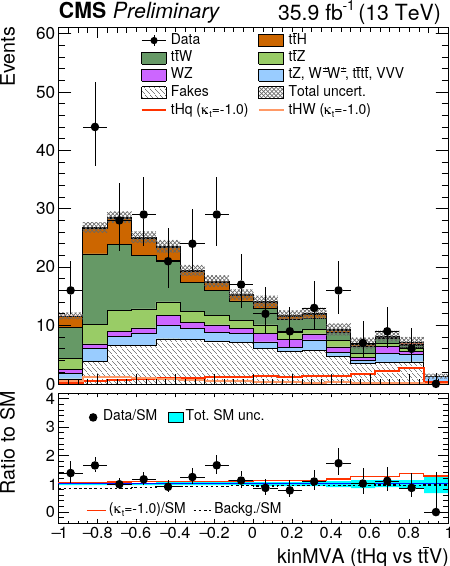
\includegraphics[scale=0.3]{figures/histo.png}
	\caption*{\tiny{Pre-fit classifier outputs for same sign dimuon, for training against $t\bar{t}V$ }}
\end{figure}
\end{minipage}
\hfill
\begin{minipage}[c]{.45\textwidth}
	\small
\begin{table}
	\centering
	\caption*{\tiny{Event yields for signal and backgrounds after the event selection for a integrated luminosity of 35.9 fb$^{-1}$. The uncertainties of yields include statistical and systematic \protect \footnotemark} }
	\begin{tabular}{cc}
		\hline
		Process & Number of events \\
		\hline
		$t\bar{t}W$ & 68 $\pm$ 10 \\
		$t\bar{t}Z$ & 25.9 $\pm$ 3.9\\
		$WZ$ & 15.1$\pm$7.7\\
		Rares & 20.9 $\pm$ 4.9\\
		Fakes & 80.9 $\pm$9.4\\
		$t\bar{t}H$ & 24.2 $\pm$ 2.1 \\
		\hline
		$tH$ (SM) & 2.14 $\pm$ 0.13\\
		$tH$ ($k_t=-1$) &26.2 $\pm$ 2.2
	\end{tabular}	
	\label{tth-table}
\end{table}
%	\begin{figure}	\centering
%	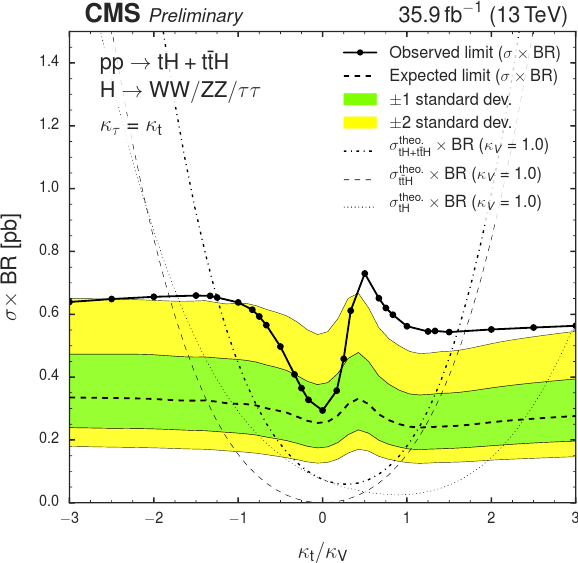
\includegraphics[width=\textwidth]{figures/sc.png}
%	\caption*{\tiny{Observed and expected 95$\%$ C.L. upper limit on the tH + t$\bar{t}$H cross section times H $\rightarrow$ WW $+$ $\tau\tau$ $+$ ZZ branching fraction for different 20 values of the coupling ratio $\kappa_t /\kappa_v$ . The expected limit is derived from a background-only MC dataset.}}
%	\end{figure}
\end{minipage}
\footnotetext{\tiny The CMS collaboration, \textit{Search for production of a Higgs boson and a single top
			quark in multilepton final states in proton collisions at 13 TeV}, CMS-HIG-18-009, Phys. Rev. D 99, 092005}
\end{frame}
}

{\nologo
\begin{frame}
\frametitle{Distribution of events in the BDT discriminant}
\begin{minipage}[b]{.48\textwidth}
\begin{figure}
	\centering
	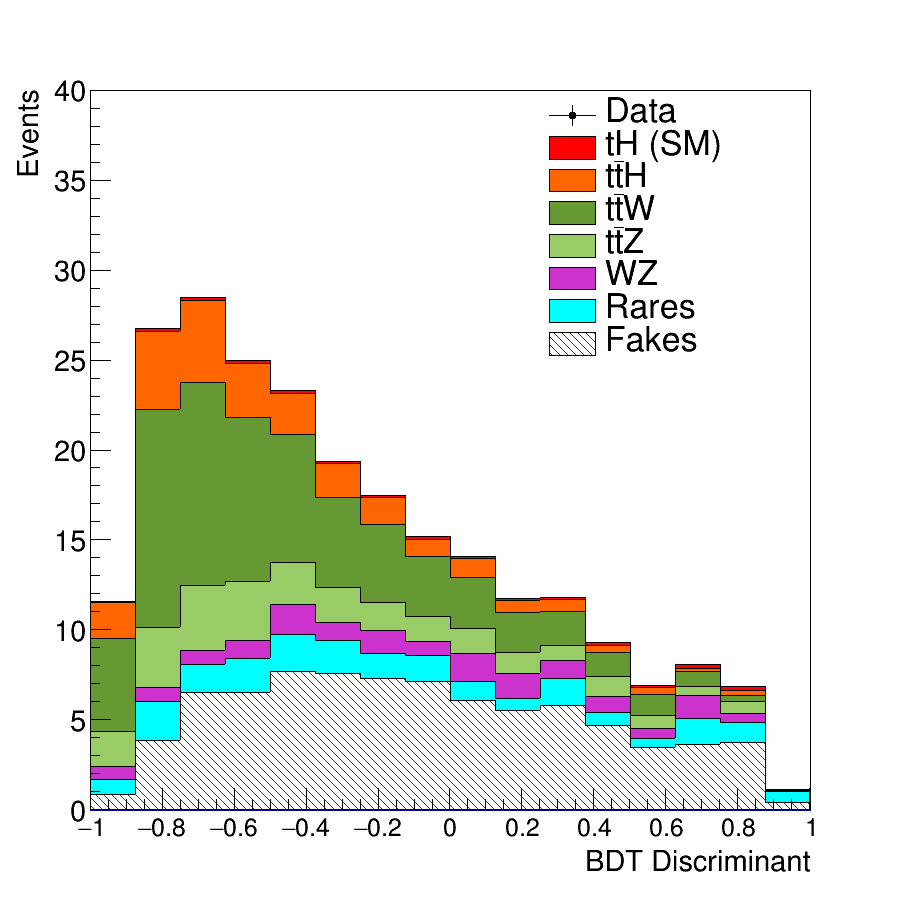
\includegraphics[width=\textwidth]{figures/kos.png}
\end{figure}
\end{minipage}
\hfill
\begin{minipage}[b]{.48\textwidth}
	\begin{figure}
		\centering
		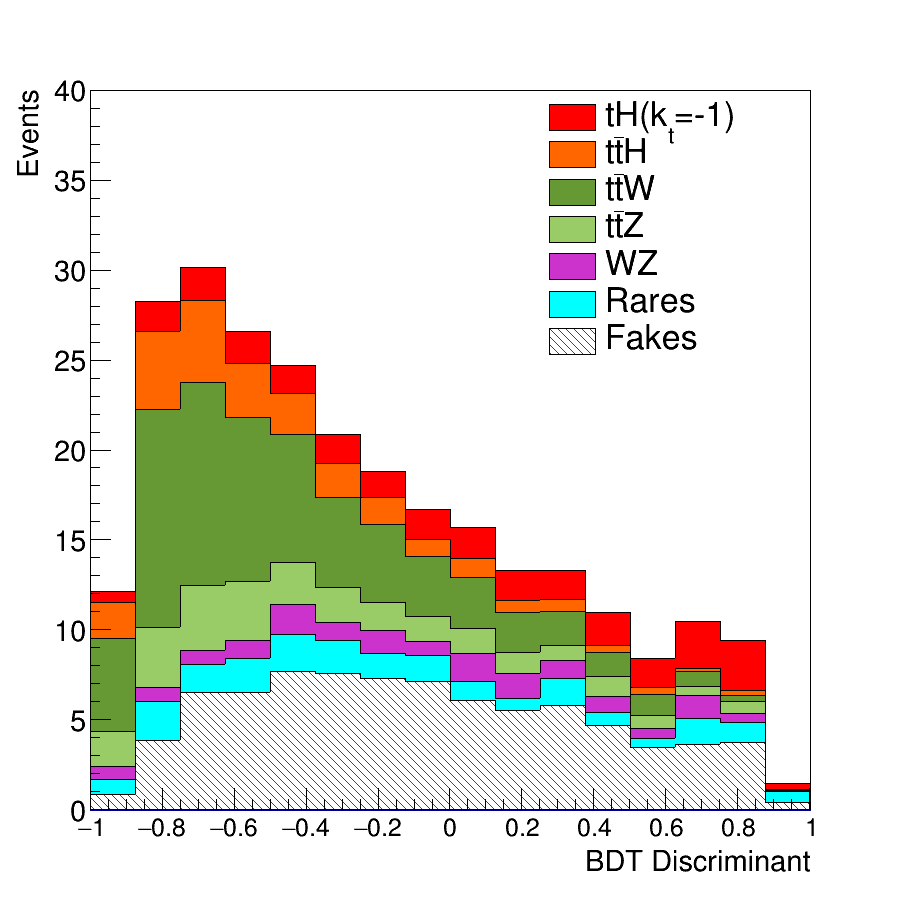
\includegraphics[width=\textwidth]{figures/kos2.png}
	\end{figure}
\end{minipage}
\begin{center}
\small{SM signal and backgrounds (Left) and $k_t$=-1 model (Right).}
\end{center}
\end{frame}
}


\begin{frame}
\subsection{Systematic uncertainties}
\frametitle{Systematic uncertainties}
\begin{itemize}
	\item The uncertainties on $t\bar{t}W$ and $t\bar{t}Z$ event yields are mainly due to the uncertainties of their production cross sections. 
	\item The uncertainty on $WZ$ background is estimated using real data events in a three lepton control region. 
	\item In the Rare backgrounds, which are not measured, a $50\%$ of uncertainty is assigned.
	\item The uncertainty on the Fakes background is estimated using real data in a control region, defined by the muon identification criteria. 
	\item For the Higgs processes $tH$ and $ttH$, the uncertainty are due to the theoretical parameters used in that simulation.
\end{itemize}

\end{frame}





\begin{frame}
\section{Statistical analysis}
\frametitle{Fitting}
	\begin{center}
	\begin{figure}
		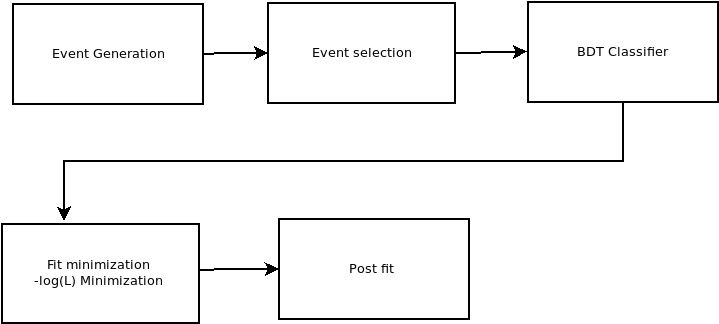
\includegraphics[width=10.5cm]{figures/fit-box.png}
		\caption*{}
	\end{figure}
\end{center}
\end{frame}

\begin{frame}
\subsection{Likelihood model}
\frametitle{Likelihood model}
{\small \begin{itemize}
\item To estimate the sensibility of the $tH$ signal, we define an Asimov dataset, made by replacing the ensemble of simulated backgrounds and signal by a single one. 
\item The statistical uncertainty of the Asimov data is calculated as $\sqrt{n}$, with $n$ the number of events.\\
\item The likelihood function is the product of Poisson probabilities for all bins
\begin{align}
	L(\mu,\alpha)=\prod_{j=1}^{N}\frac{(\mu s_j +b_j)^{n_j}}{n_j !}e^{-(\mu s_j+b_j)} \prod_{k=1}^M e^{\frac{-\alpha^2_k}{2}}
\end{align}
	where $N$ is the total number of bins, $n_j$ is the number of events in a bin $j$, $s_j$ is the number of signal events, $\mu$ is a parameter that modifies the signal strength and $b_j$ is the number of background events.
\end{itemize}}
\end{frame}


\begin{frame}
\frametitle{Likelihood model}
{\small
\begin{itemize}
	\item $b_j$ is the sum of different background processes $k$
	\begin{align}
	b_j=\sum_k^M b_j^k(1+ \alpha_k \sigma_k)
	\end{align}
	$\alpha_k$ is the parameter that modifies the expected background prediction and $\sigma_k$ is the systematic uncertainty of the associated background. $\sigma_k$ for the backgrounds are shown in the Table of yields. 
		\item The fit is applied by minimizing the $-\log{L}$ (NLL) with respect to the parameter $\mu$ and $\alpha_k$. The minimization is performed by using the package ROOFIT. In the next slides, it shows the results of the model fitting using the Asimov data for the SM and the $k_t=-1$.
\end{itemize}}
\end{frame}

\begin{frame}
\subsection{Results}
\frametitle{Results}
\begin{minipage}{0.4\textwidth}
	\begin{center}
	\begin{figure}
		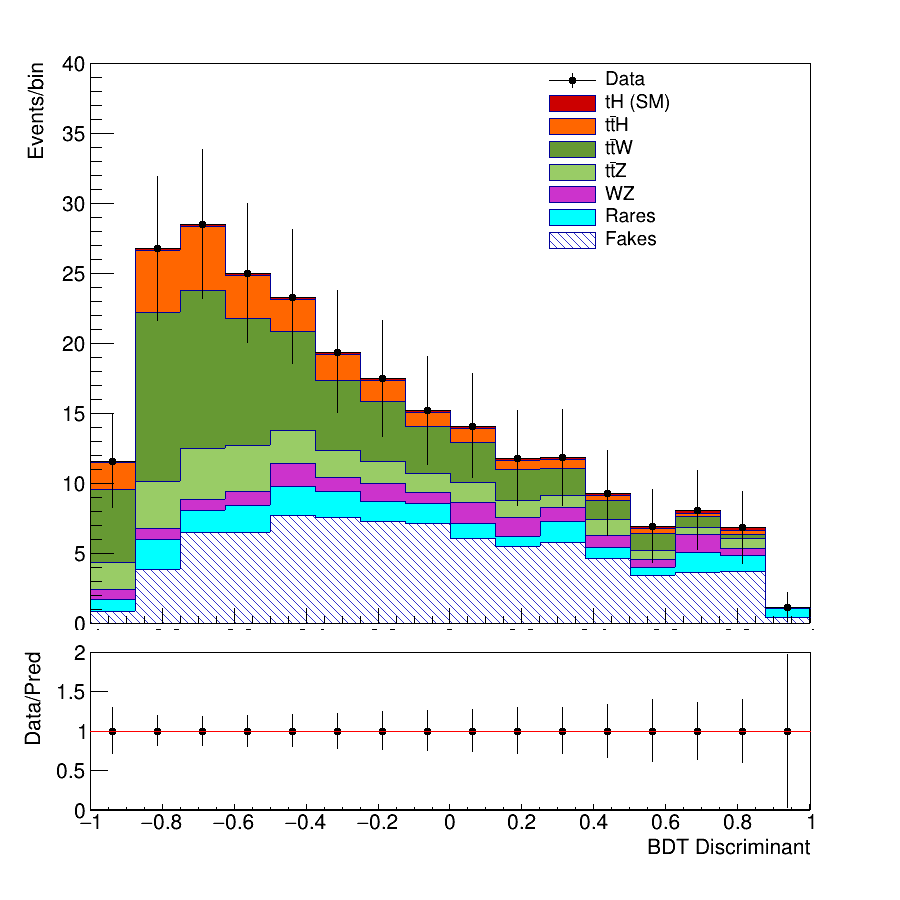
\includegraphics[width=5.5cm,height=5cm]{figures/simple.png}
		\caption*{\tiny{Post-fit signal and background yields for tH process in the SM. In the
			box below each distribution, the ratio of the observed and  event yields is shown}}
	\end{figure}
\end{center}
\end{minipage}\hfill \quad
\begin{minipage}{0.4\textwidth}
	\begin{center}
	\begin{figure}
		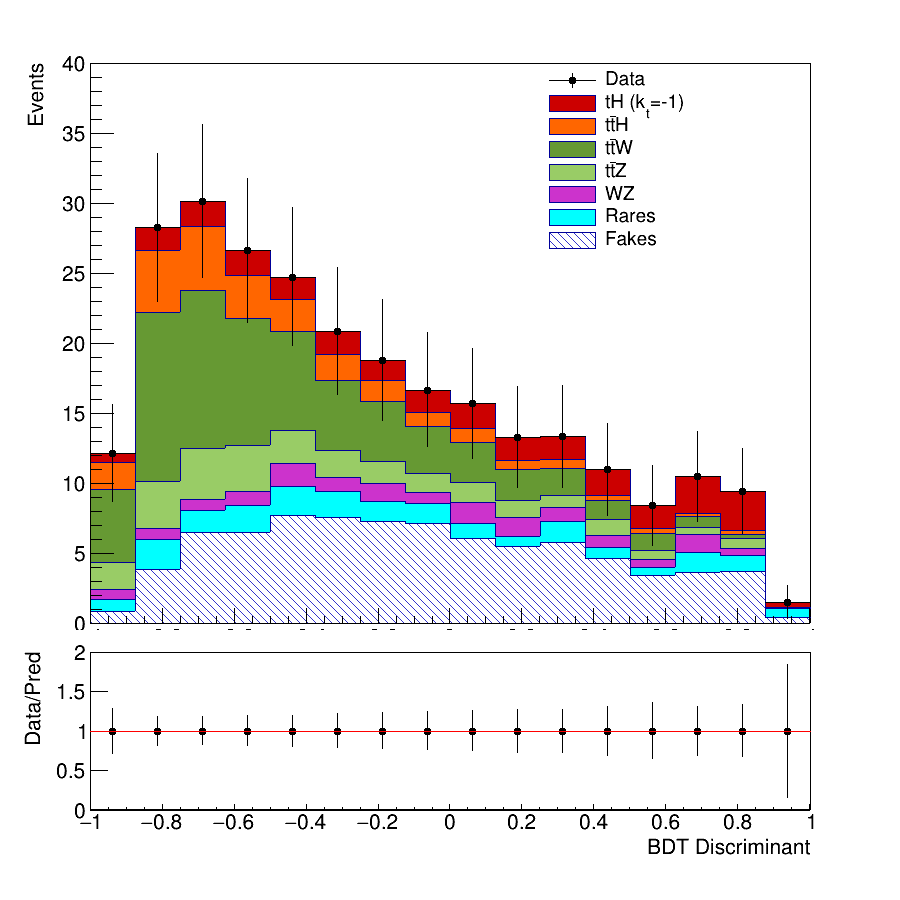
\includegraphics[width=5.5cm,height=5cm]{figures/simple-kt-1.png}
		\caption*{\tiny{Post-fit signal and background yields for tH process in the $k_t$=-1. 
	In the box below each distribution, the ratio of the observed and event yields is shown}}
	\end{figure}
\end{center}
\end{minipage}
\end{frame}


\begin{frame}
\section{Results}
\frametitle{Results}
	\begin{table}[ht!]
		\centering
		\caption*{Postfit yields for the fit to the Asimov data corresponding to 35.9 fb$^{-1}$. The uncertainty given is the combined statistical plus systematic.}
		\begin{tabular}{ccc}
			\hline
			Process & SM & $k_{t}$=-1 \\
			\hline
			$t\bar{t}W$ & 68$\pm$8.9& 68 $\pm$8.9 \\
			$t\bar{t}Z$ & 25.9$\pm$3.8&25.9$\pm$3.8\\
			$WZ$ & 15.1$\pm$7.4& 15.1$\pm$7.4\\
			Rares & 20.8$\pm$4.8& 20.8$\pm$4.8 \\
			Fakes & 80.9$\pm$9.0& 80.9$\pm$8.9 \\
			$t\bar{t}H$ & 24.2$\pm$2.0 & 24.2$\pm$2.0 \\
			\hline
			$tH$& 2.1$\pm$16.5 &26.2$\pm$13.1 
		\end{tabular}
		\label{table1}
	\end{table}
 Prefit uncertainty is statistical only. Postfit uncertainty is statistical + systematic.
\end{frame}



\begin{frame}
\frametitle{Results}
\framesubtitle{Likelihood scan}
{\small
	\begin{itemize}
\item Due to the large background, the signal strength for the Asimov data with 35.9 fb$^{-1}$ is consistent with zero.
Therefore, we estimate an upper limit on the signal strength at 95$\%$ confidence level.
\item We can define the likelihood ratio
\begin{align}
\lambda(\mu,\alpha)=\frac{L(\mu,\alpha)}{L(\hat{\mu},\hat{\alpha})}
\end{align}
Where $\hat{\alpha}$ and $\hat{\mu}$ are the parameters obtained in the previous section which correspond to the minimal of the NLL.
\item To determine an upper limit on the strength parameter $\mu$, we use the following statistical test
\begin{align}
q(\mu,\alpha)= -2\ln{\lambda} 
\end{align}
\item High values of $q$ represent greater incompatibility between the data and the fit model.
$q$ is a random variable with a $\chi^2$ distribution.
\end{itemize}
}
\end{frame}


\begin{frame}
\frametitle{Results}
\framesubtitle{Likelihood scan for an integrated luminosity of 35.9 fb$^{-1}$}
\begin{minipage}{0.5\textwidth}
	\begin{center}
		\begin{figure}
			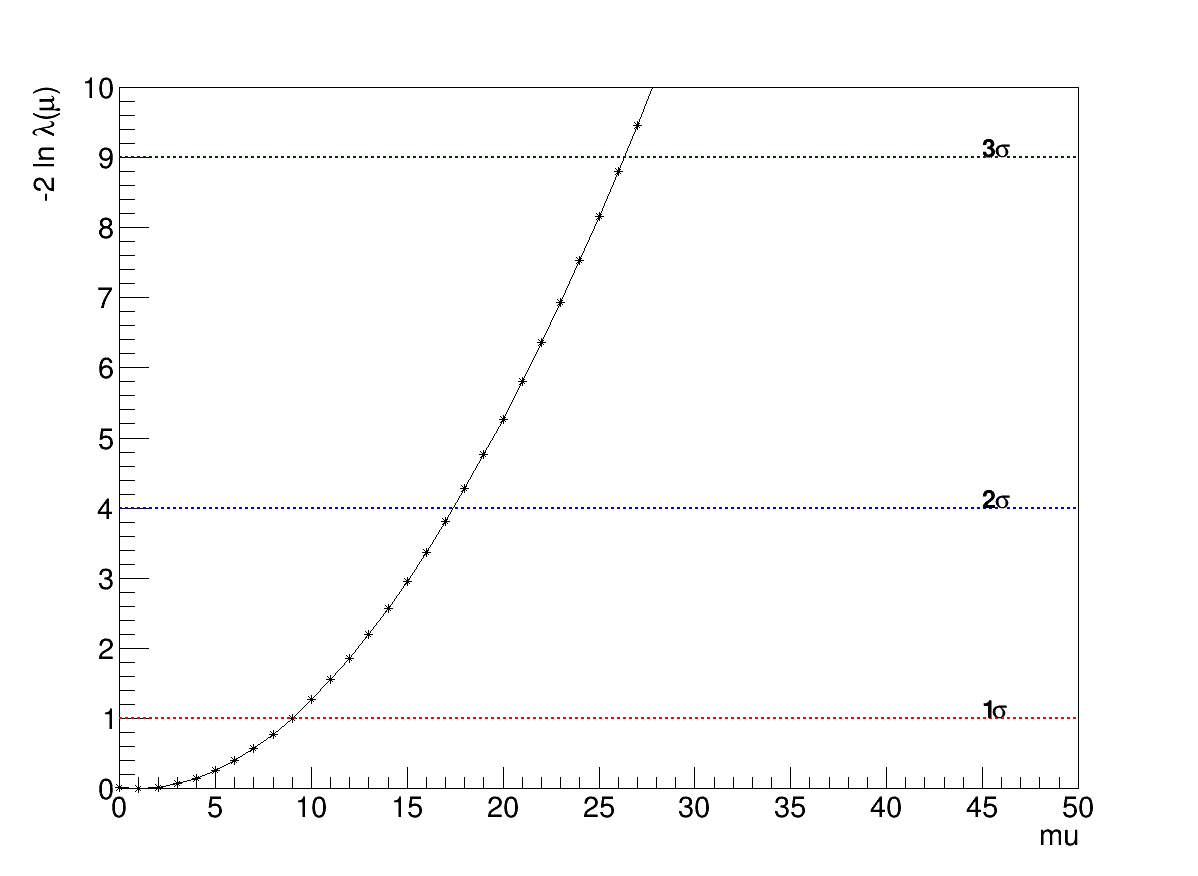
\includegraphics[width=6cm,height=5cm]{figures/Likelihood.png}
			\caption*{Likelihood scan for k$_t$=1 (SM)}
		\end{figure}
	\end{center}
\end{minipage}\hfill
\begin{minipage}{0.5\textwidth}
	\begin{center}
		\begin{figure}
			\includegraphics[width=6cm,height=5cm]{figures/kt-1/Likelihood-kt-1.png}
			\caption*{Likelihood scan for k$_t$=-1}
		\end{figure}
	\end{center}
\end{minipage}
\end{frame}


{\nologo
	\begin{frame}
	\frametitle{Extrapolation of luminosity for SM }
	\begin{center}
		\begin{tabular}{cc}
			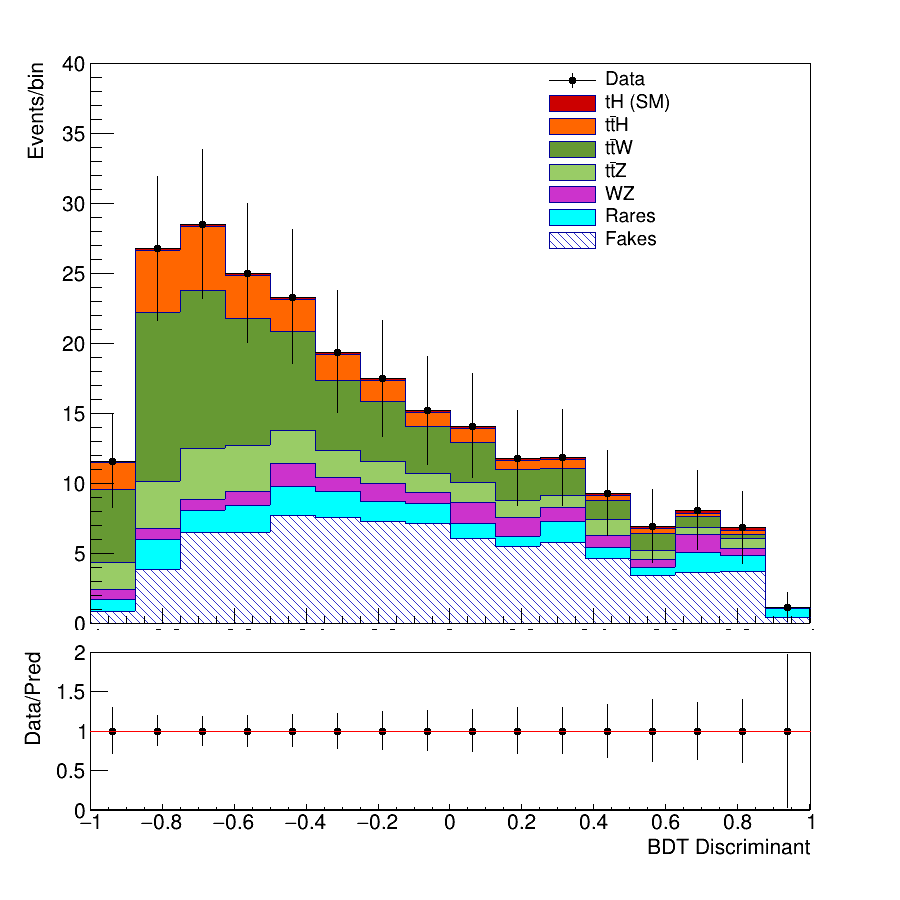
\includegraphics[width=5.5cm,height=3cm]{figures/simple.png} &
			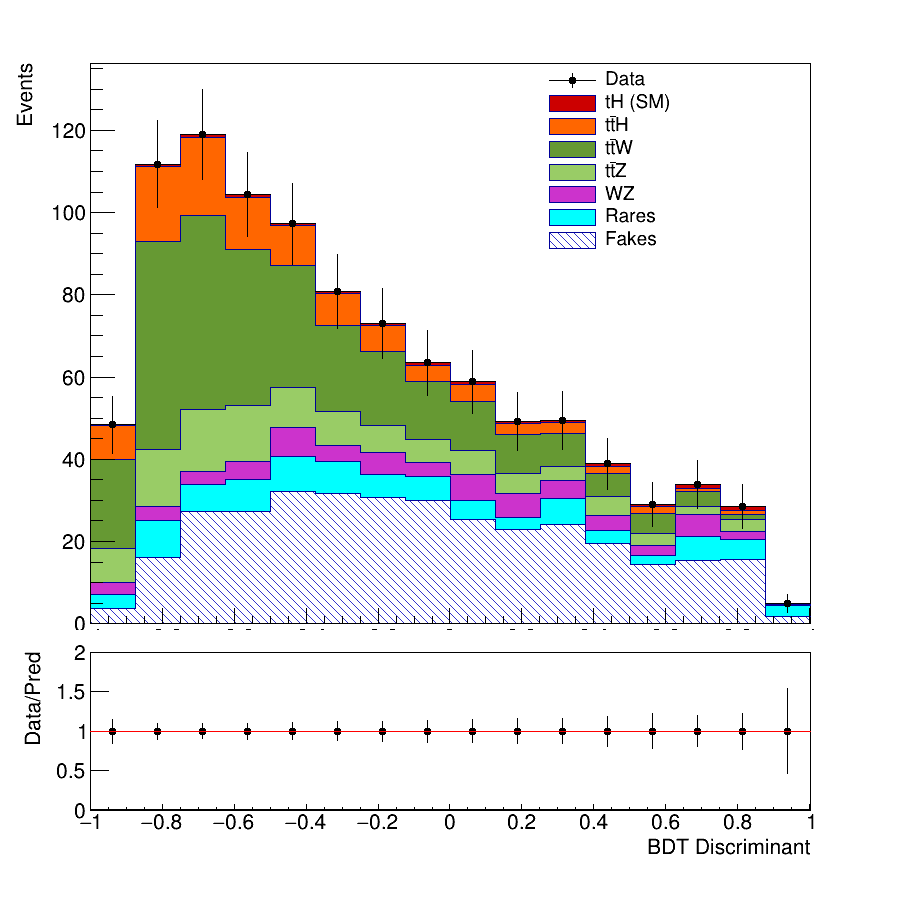
\includegraphics[width=5.5cm,height=3cm]{figures/150fb/simple-150.png}\\ 
			\scriptsize{35.9 fb$^{-1}$} & \scriptsize{150 fb$^{-1}$} \\
			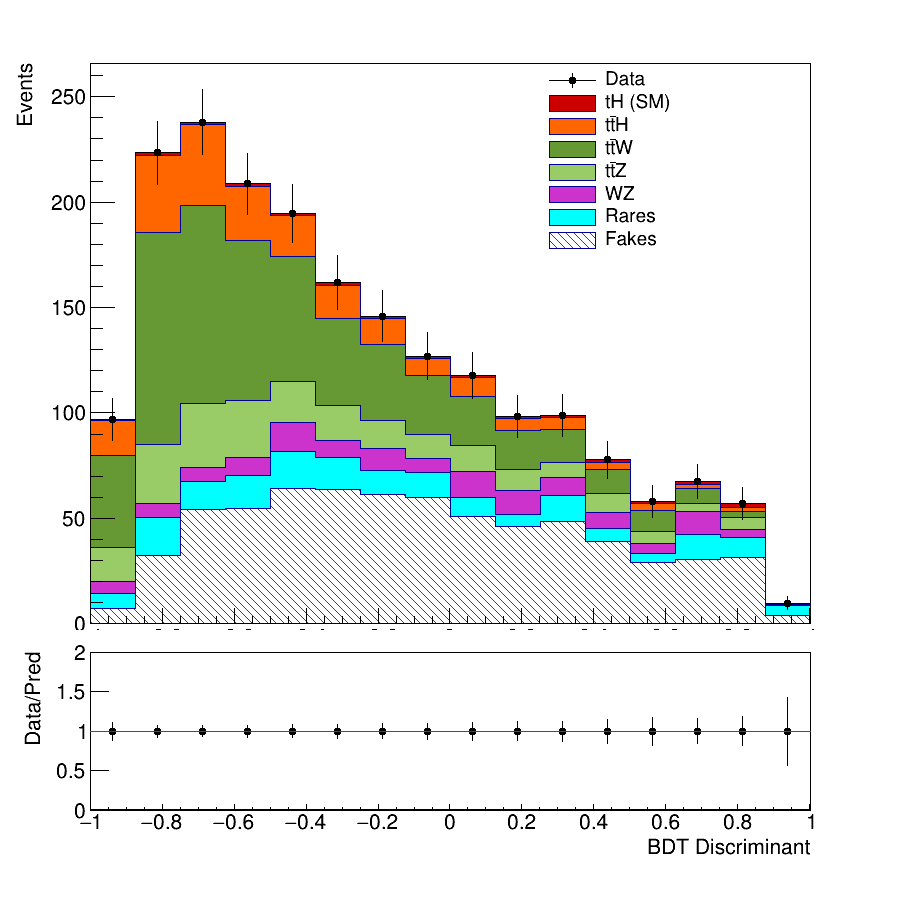
\includegraphics[width=5.5cm,height=3cm]{figures/300fb/simple-300.png}&
			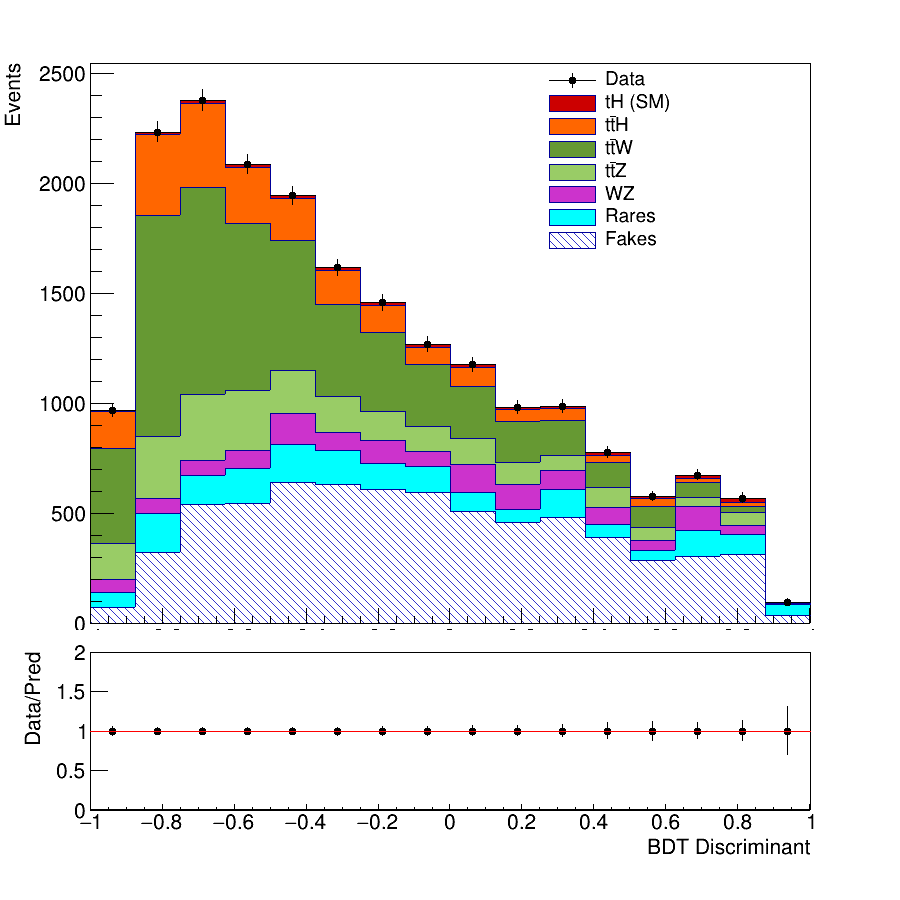
\includegraphics[width=5.5cm,height=3cm]{figures/3000fb/simple-3000.png}\\
			\scriptsize{300 fb$^{-1}$} & \scriptsize{3000 fb$^{-1}$} \\
		\end{tabular}
	\end{center}
\end{frame}
}

{\nologo
	\begin{frame}
	\frametitle{Likelihood scan for SM }
	\begin{center}
		\begin{tabular}{cc}
			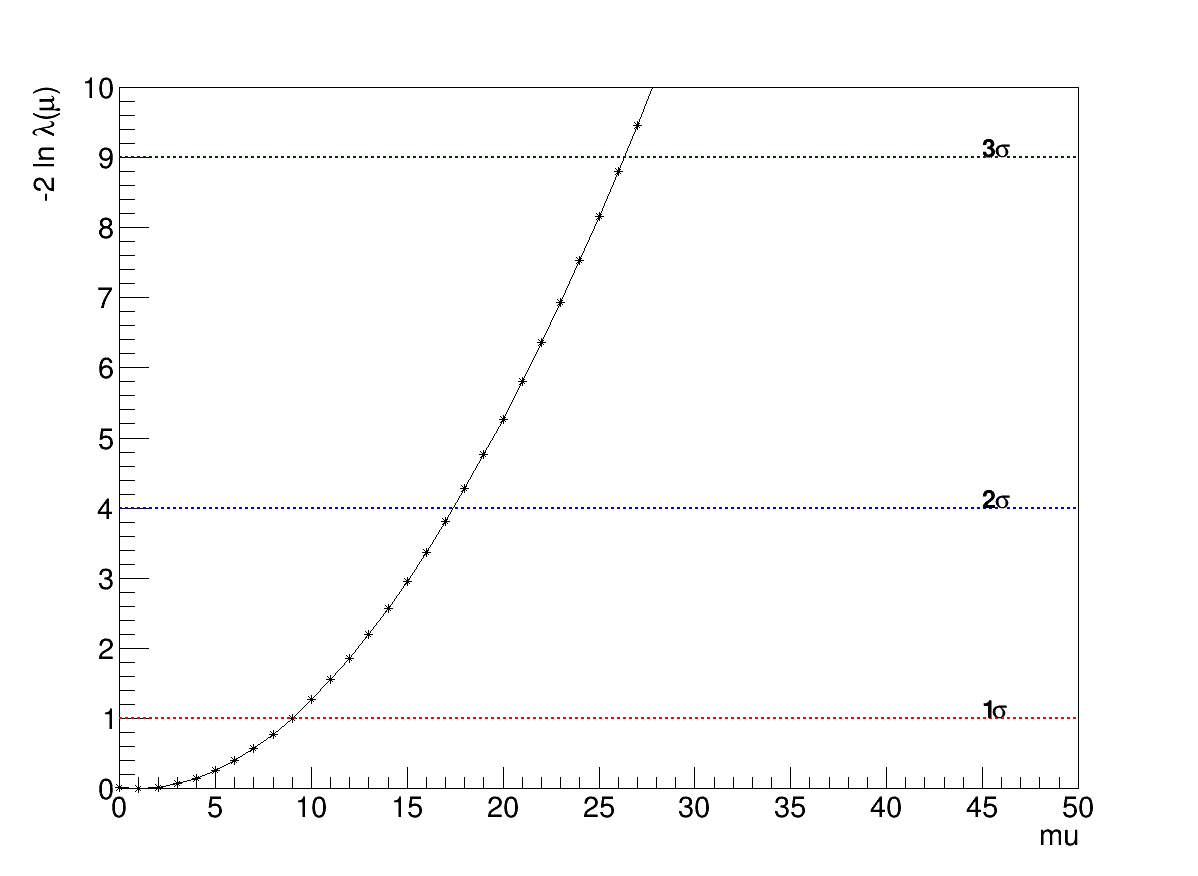
\includegraphics[width=5.5cm,height=3cm]{figures/Likelihood.png} &
			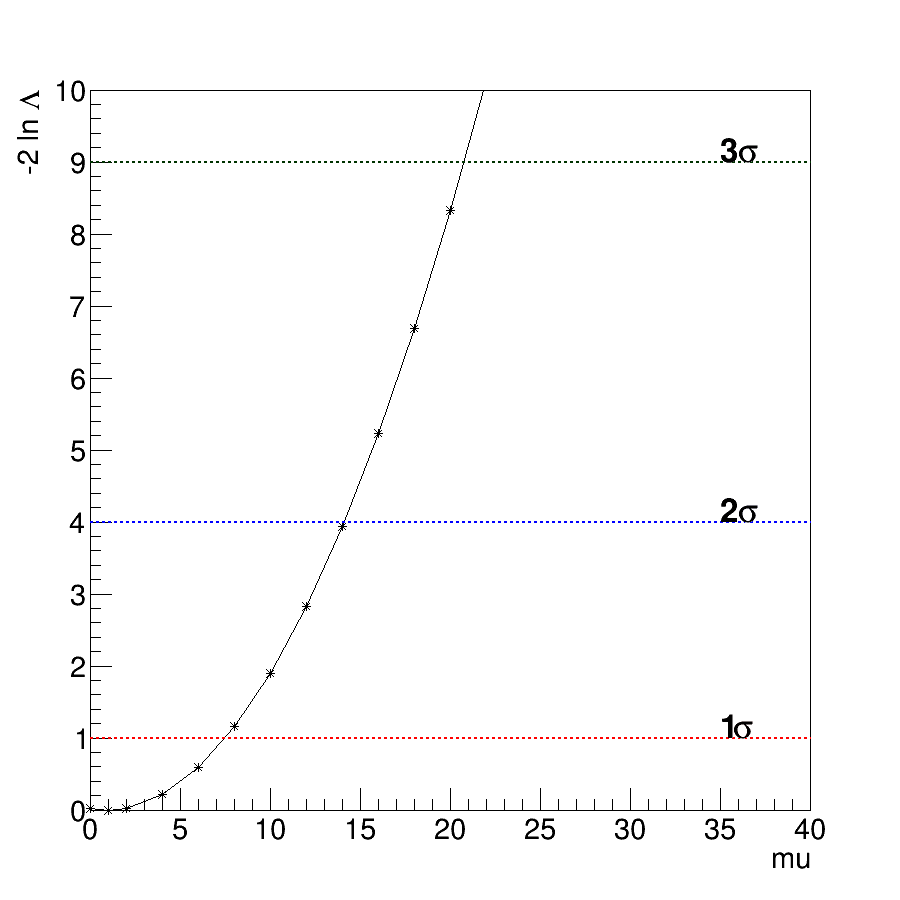
\includegraphics[width=5.5cm,height=3cm]{figures/150fb/Likelihood.png}\\ 
			\scriptsize{35.9 fb$^{-1}$} & \scriptsize{150 fb$^{-1}$} \\
			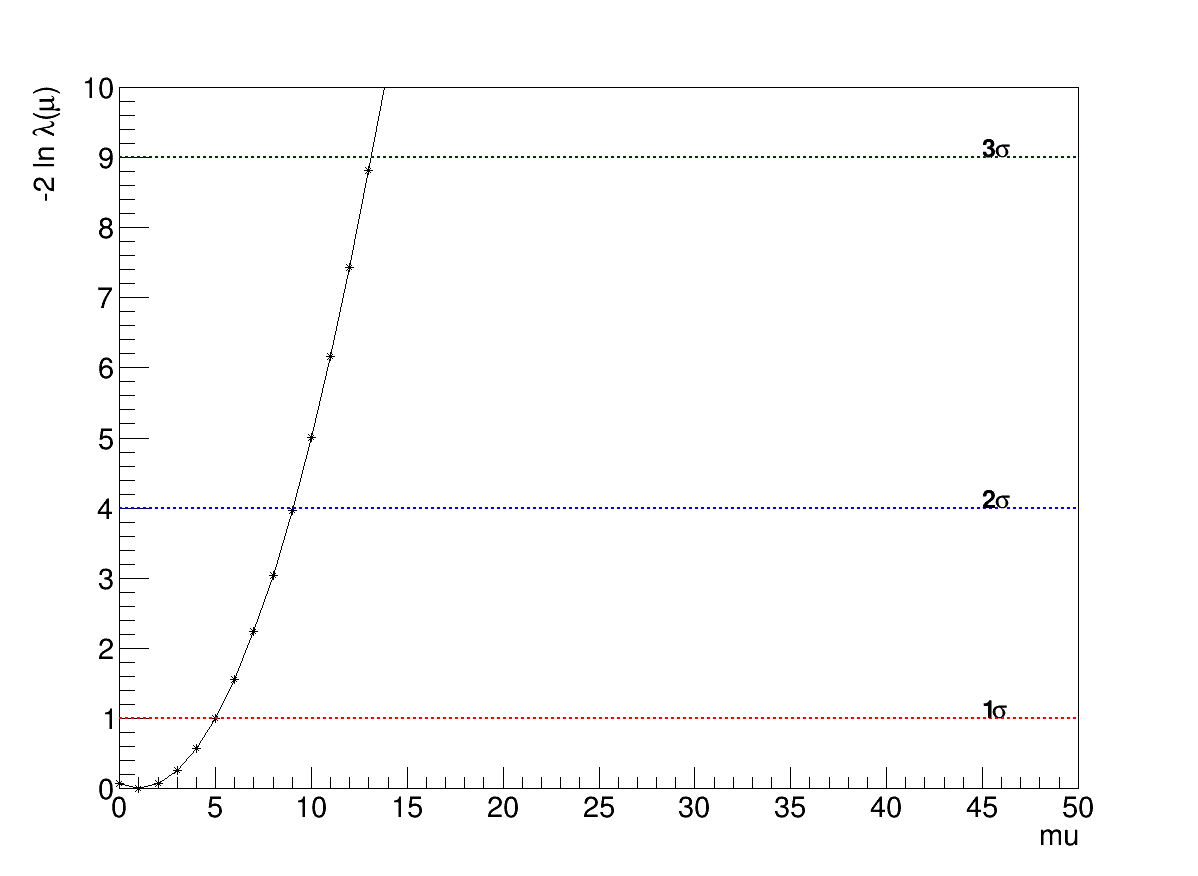
\includegraphics[width=5.5cm,height=3cm]{figures/300fb/Likelihood.png}&
			\includegraphics[width=5.5cm,height=3cm]{figures/3000fb/Likelihood.png}\\
			\scriptsize{300 fb$^{-1}$} & \scriptsize{3000 fb$^{-1}$} \\
		\end{tabular}
	\end{center}
\end{frame}
}


{\nologo
	\begin{frame}
	\frametitle{Extrapolation of luminosity for $k_t=-1$}
	\begin{center}
		\begin{tabular}{cc}
			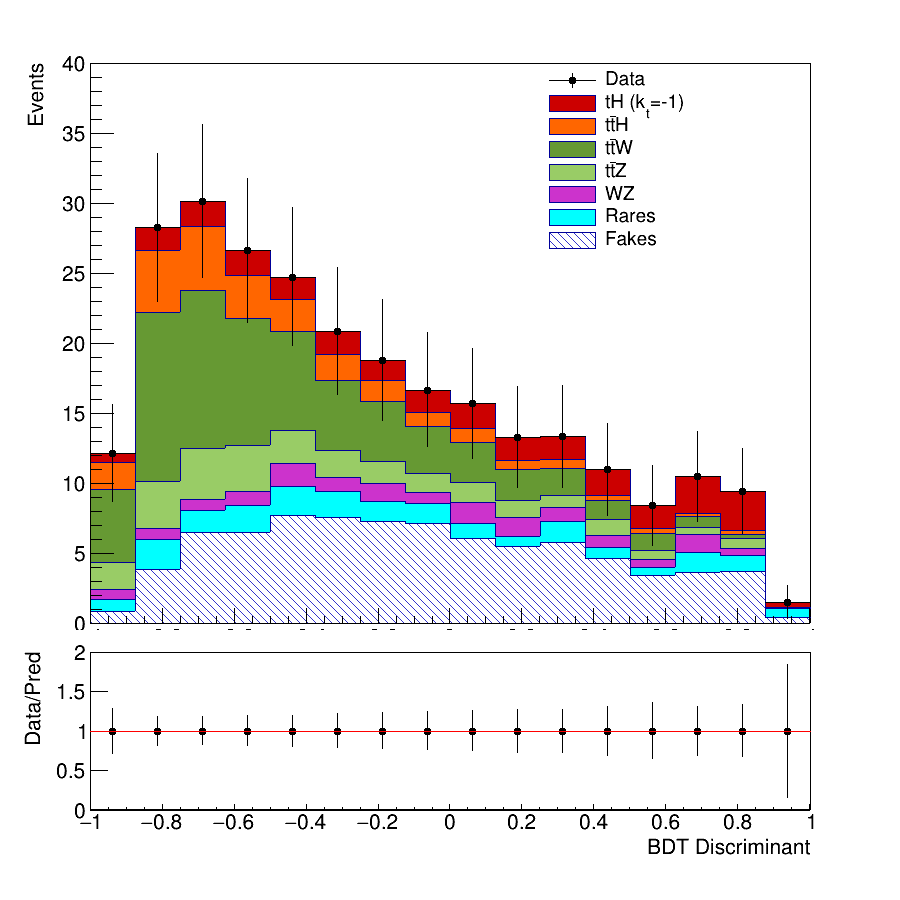
\includegraphics[width=5.5cm,height=3cm]{figures/simple-kt-1.png} &
			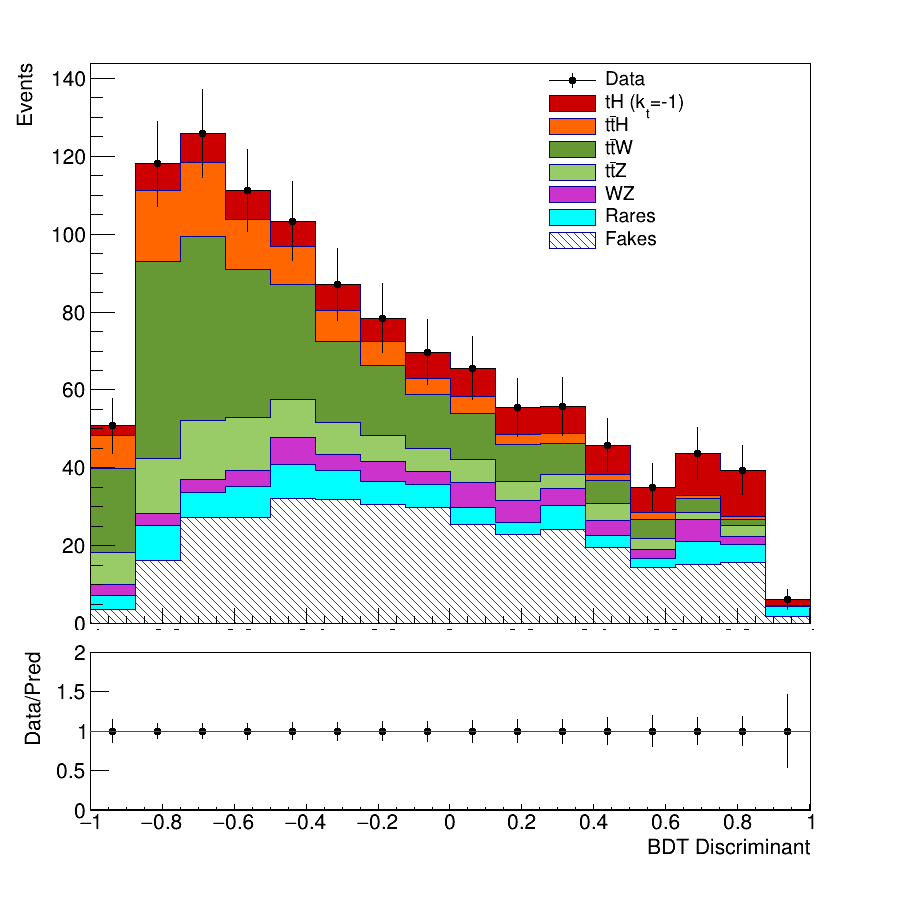
\includegraphics[width=5.5cm,height=3cm]{figures/kt-1/150fb/simple-150-kt-1.png}\\ 
			\scriptsize{35.9 fb$^{-1}$} & \scriptsize{150 fb$^{-1}$} \\
			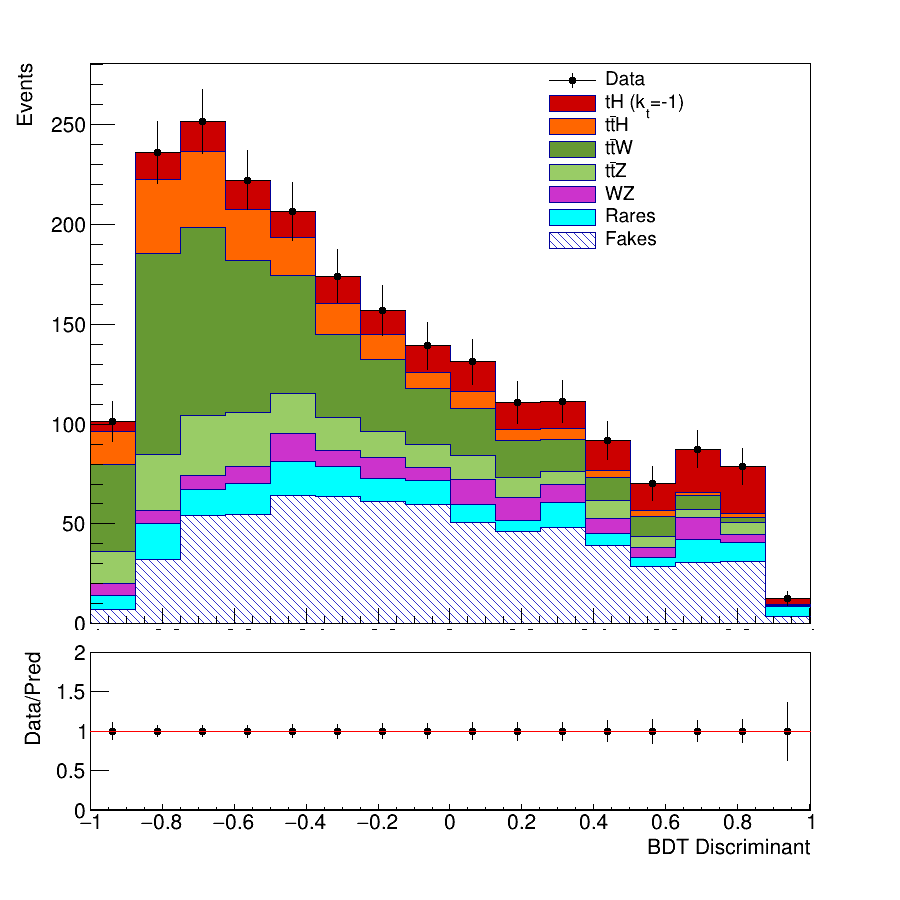
\includegraphics[width=5.5cm,height=3cm]{figures/kt-1/300fb/simple-300-kt-1.png}&
			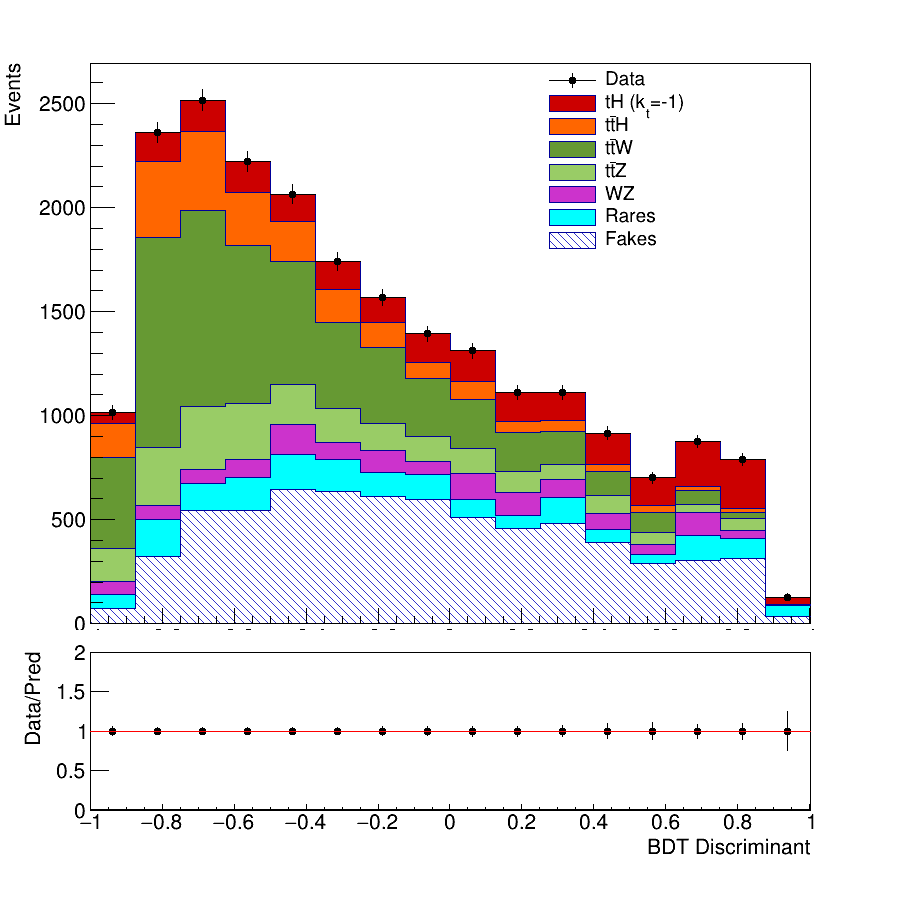
\includegraphics[width=5.5cm,height=3cm]{figures/kt-1/3000fb/simple-3000-kt-1.png}\\
			\scriptsize{300 fb$^{-1}$} & \scriptsize{3000 fb$^{-1}$} \\
		\end{tabular}
	\end{center}
\end{frame}
}


{\nologo
	\begin{frame}
	\frametitle{Likelihood scan for  $k_t=-1$}
	\begin{center}
		\begin{tabular}{cc}
			\includegraphics[width=5.5cm,height=3cm]{figures/kt-1/35.9fb/Likelihood-kt-1.png} &
			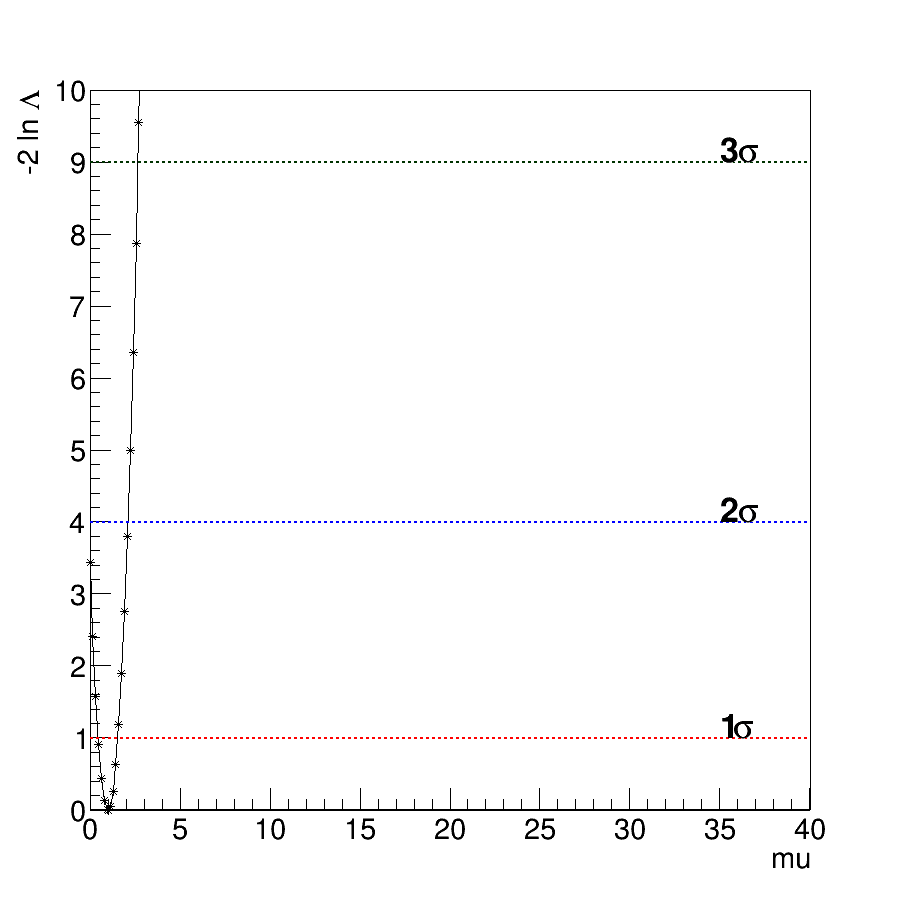
\includegraphics[width=5.5cm,height=3cm]{figures/kt-1/150fb/Likelihood.png}\\ 
			\scriptsize{35.9 fb$^{-1}$} & \scriptsize{150 fb$^{-1}$} \\
			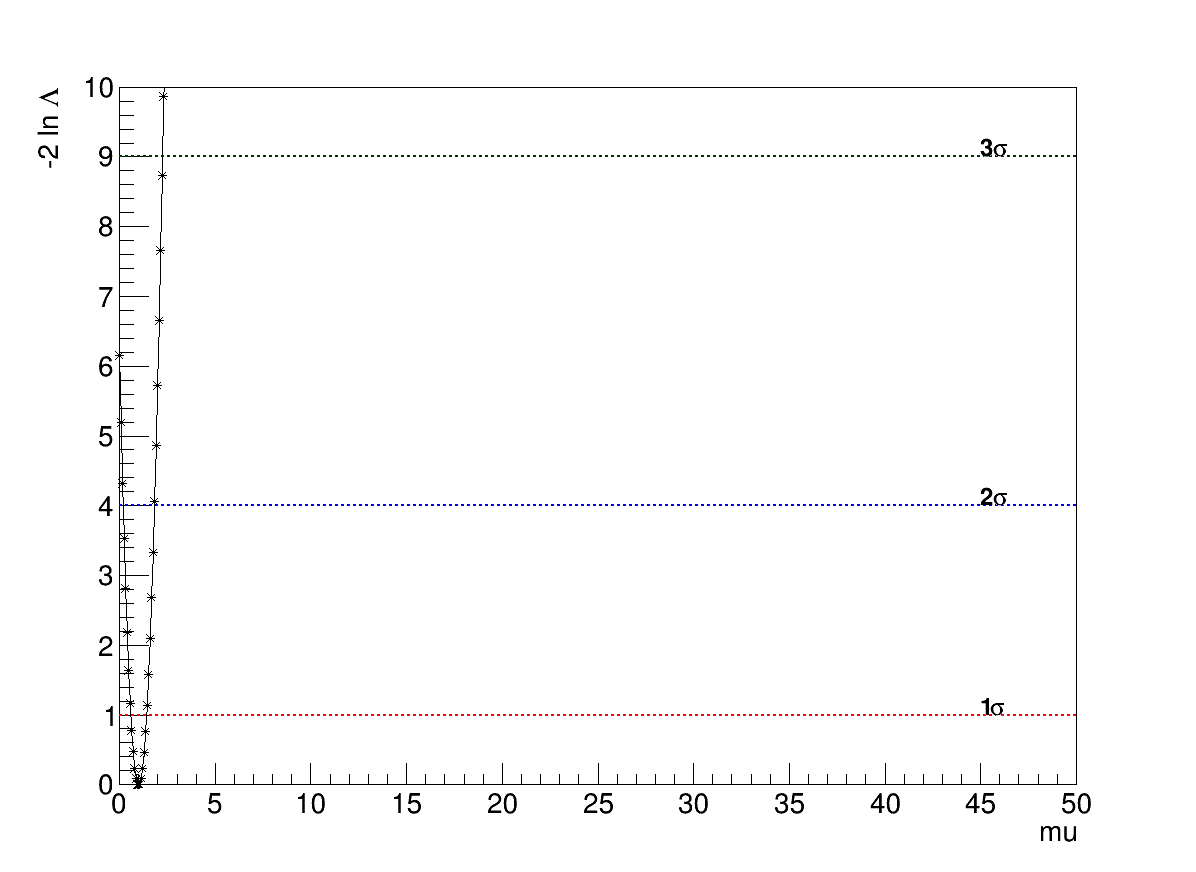
\includegraphics[width=5.5cm,height=3cm]{figures/kt-1/300fb/Likelihood.png}&
			\includegraphics[width=5.5cm,height=3cm]{figures/kt-1/3000fb/Likelihood.png}\\
			\scriptsize{300 fb$^{-1}$} & \scriptsize{3000 fb$^{-1}$} \\
		\end{tabular}
	\end{center}
\end{frame}
}



\begin{frame}
\frametitle{Results}
\framesubtitle{Upper limit}
\tiny{
\begin{table}[ht!]
	\caption*{Results of $\mu$ and upper limits for Asimov extrapolations for SM and $k_t$=-1 models.}
	\begin{tabular}{|c|c|c|c|c|}
		\hline
		Luminosity (fb$^{-1}$)	&$\mu$ (SM) &$\mu$ (SM) upper limit & $\mu$ ($k_t$=-1) &$\mu$ ($k_t$=-1) upper limit \\
		\hline
		35.9 & 1.0 $\pm$ 7.7 & 17 & 1.0 $\pm$ 0.5 & 2.3 \\
		\hline
		150& 1.0 $\pm$ 6.7& 11 & 1.0 $\pm$ 0.4 &1.8\\
		\hline
		300&1.0 $\pm$ 4.3 &8.7 & 1.0 $\pm$ 0.3 &1.5 \\
		\hline
		3000&1.0 $\pm$ 1.7 & 4.3 &	 1.0 $\pm$ 0.1 & 1.1\\
		\hline
	\end{tabular}
	\label{upper}
\end{table}
}
\end{frame}


%\begin{frame}
%\section{Conclusions}
%\frametitle{Conclusions}
%\begin{itemize}
%	\item We analyzed the $tH$ process produced from PP collisions for the production of $\mu\mu$ final states   
%	\item We discussed about events selections for the 2016 Run 2 from CMS.
%	\item The creation of an Asimov model with systematic uncertainties to make a minimization (fit) and obtain a fit which is compatible with Standard Model.
%	\item Generation of likelihood scan for the exclusion of data and obtain the probability of detection of a Higgs boson.
%	\item Generating simulations for predict results with higher luminosities, according to the future experiments. 
%\end{itemize}
%\end{frame}

\begin{frame}
\frametitle{Conclusions}
\begin{itemize}
\item The results of the analysis for the SM case indicates that it is impossible to detect a Higgs boson using same sign dimuon channel in the $tH$ process due to the low number of events and a huge uncertainty.
\item For the SM scenario the expected uncertainty even at the largest luminosities is not enough to observe the signal and only an upper limit can be placed.
\item For the $k_t$=-1, the uncertainty is low due to higher number of events for $tH$ process and it is possible to detect a Higgs boson, but this model is purely theoretical.
\item It requires a new analysis that includes more channels such as three leptons in the final state for improve the sensibility of the signal.
\end{itemize}
\end{frame}


	\begin{thebibliography}{99}
		\bibliographystyle{unsrt}
	\begin{frame}
	\tiny
%	\section{References}
	\frametitle{References}
	\bibliographystyle{amsalpha}
	\bibitem{1}Gross F. \textit{Relativistic quantum mechanics and field theory}, 1994 ,WllEY-VCH Verlag GmbH \& Co. KGaA
	\bibitem{2} Griffiths, D. \textit{Introduction to Elementary Particles}, $2^\frac{\circ}{}$ edition, 2008,WllEY-VCH Verlag GmbH \& Co. KGaA
		\bibitem{2}The CMS collaboration, \textit{Search for production of a Higgs boson and a single top
	quark in multilepton final states in proton collisions at 13 TeV}, CMS-HIG-18-009, Phys. Rev. D 99, 092005
	\bibitem{3}Verkerke W \textit{Dealing with systematic uncertainties} 2014. From
\url{https://indico.cern.ch/event/287744/contributions/1641261/attachments/535763/738679/Verkerke_Statistics_3.pdf}
\bibitem{5} ATLAS and CMS
Collaborations, \textit{Combined measurement of the Higgs boson mass in
	pp collisions at $\sqrt{s}$= 7 and 8 TeV with the ATLAS and CMS experiments}, Phys. Rev. Lett.
114 (2015) doi:10.1103/PhysRevLett.114.191803, arXiv:1503.07589
\bibitem{4} Cowan G. , Cranmer K., Gross E. , Vitells O.\textit{ Asymptotic formulae for
	likelihood-based tests of new physics} 2013 , arXiv:1007.1727
\bibitem{7}CMS collaboration \textit{Search for tHq production in multilepton final states at 13 TeV} ,2017,CMS AN-16-378
\bibitem{6}CMS collaboration \textit{High-Luminosity Large Hadron Collider (HL-LHC)}, 2017,CERN-2017-007-M
\end{frame}
\end{thebibliography}

\begin{frame}
\section{Supportive slides}
\huge{Back up}
\end{frame}

{\nologo
	\begin{frame}
		\Fontvi
		\begin{center}
			\begin{tabular}{cc}
				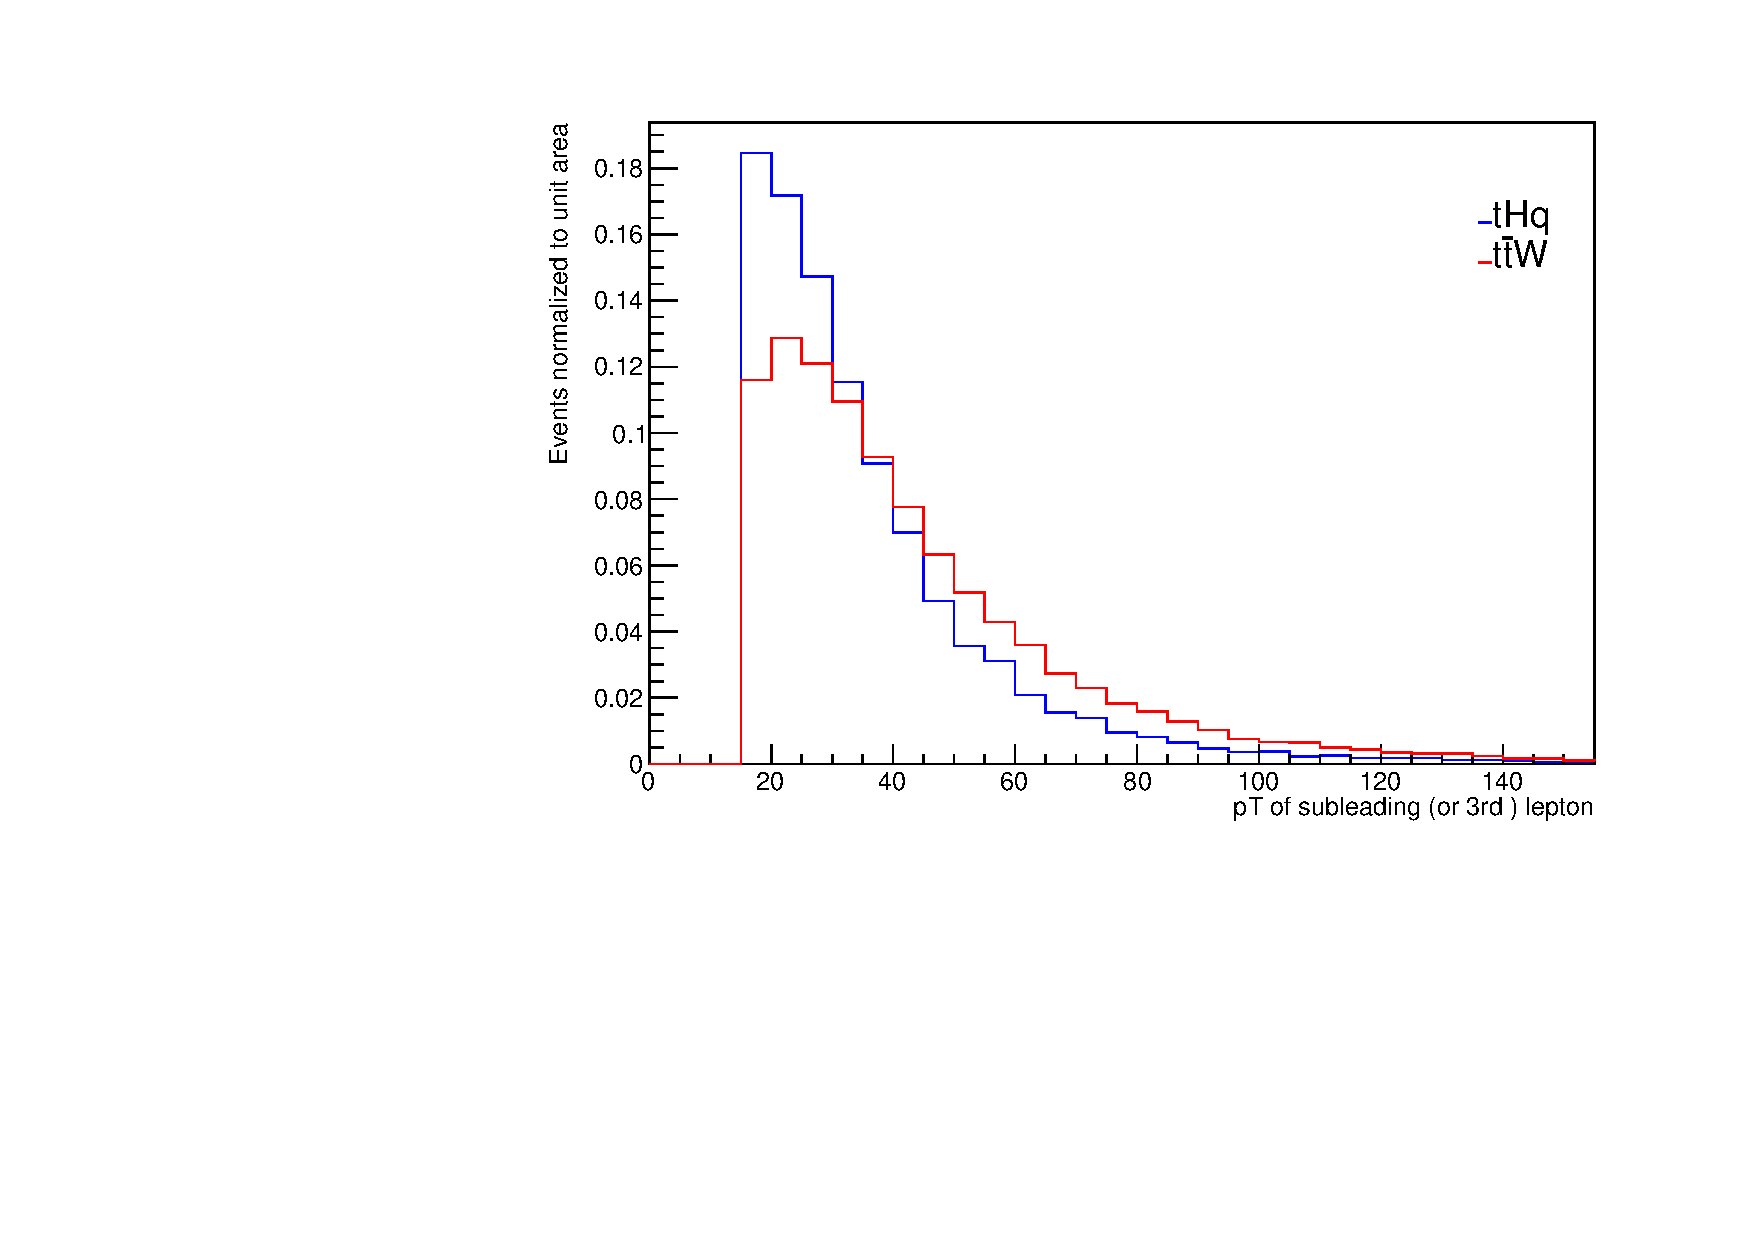
\includegraphics[width=5.5cm,height=3cm]{figures/distributions/compare_variables-pt-sub} &
				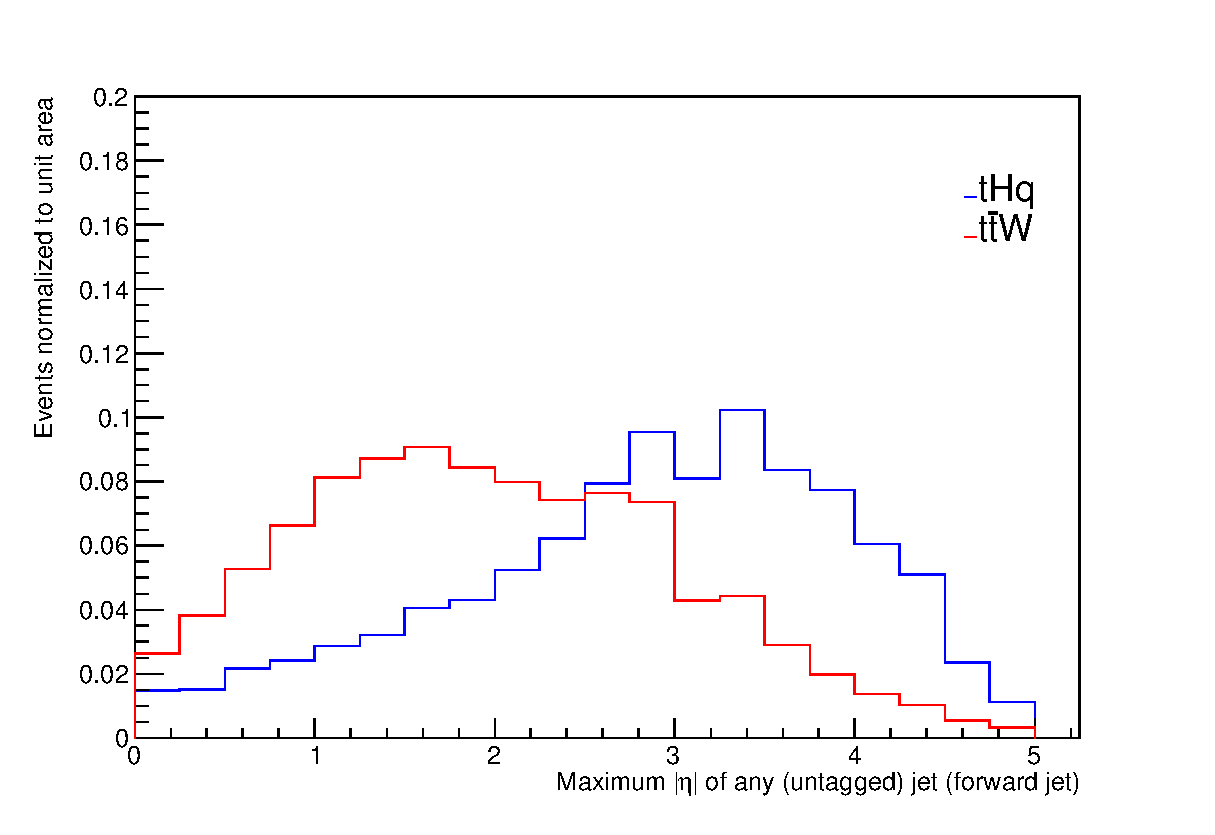
\includegraphics[width=5.5cm,height=3cm]{figures/distributions/compare_variables-abs-pj-eta}\\ 
				{Distribution of events of pt of the sub leading leptons} &{Distribution of selected events as a function of the jet with largest value of $|\eta|$}\\
				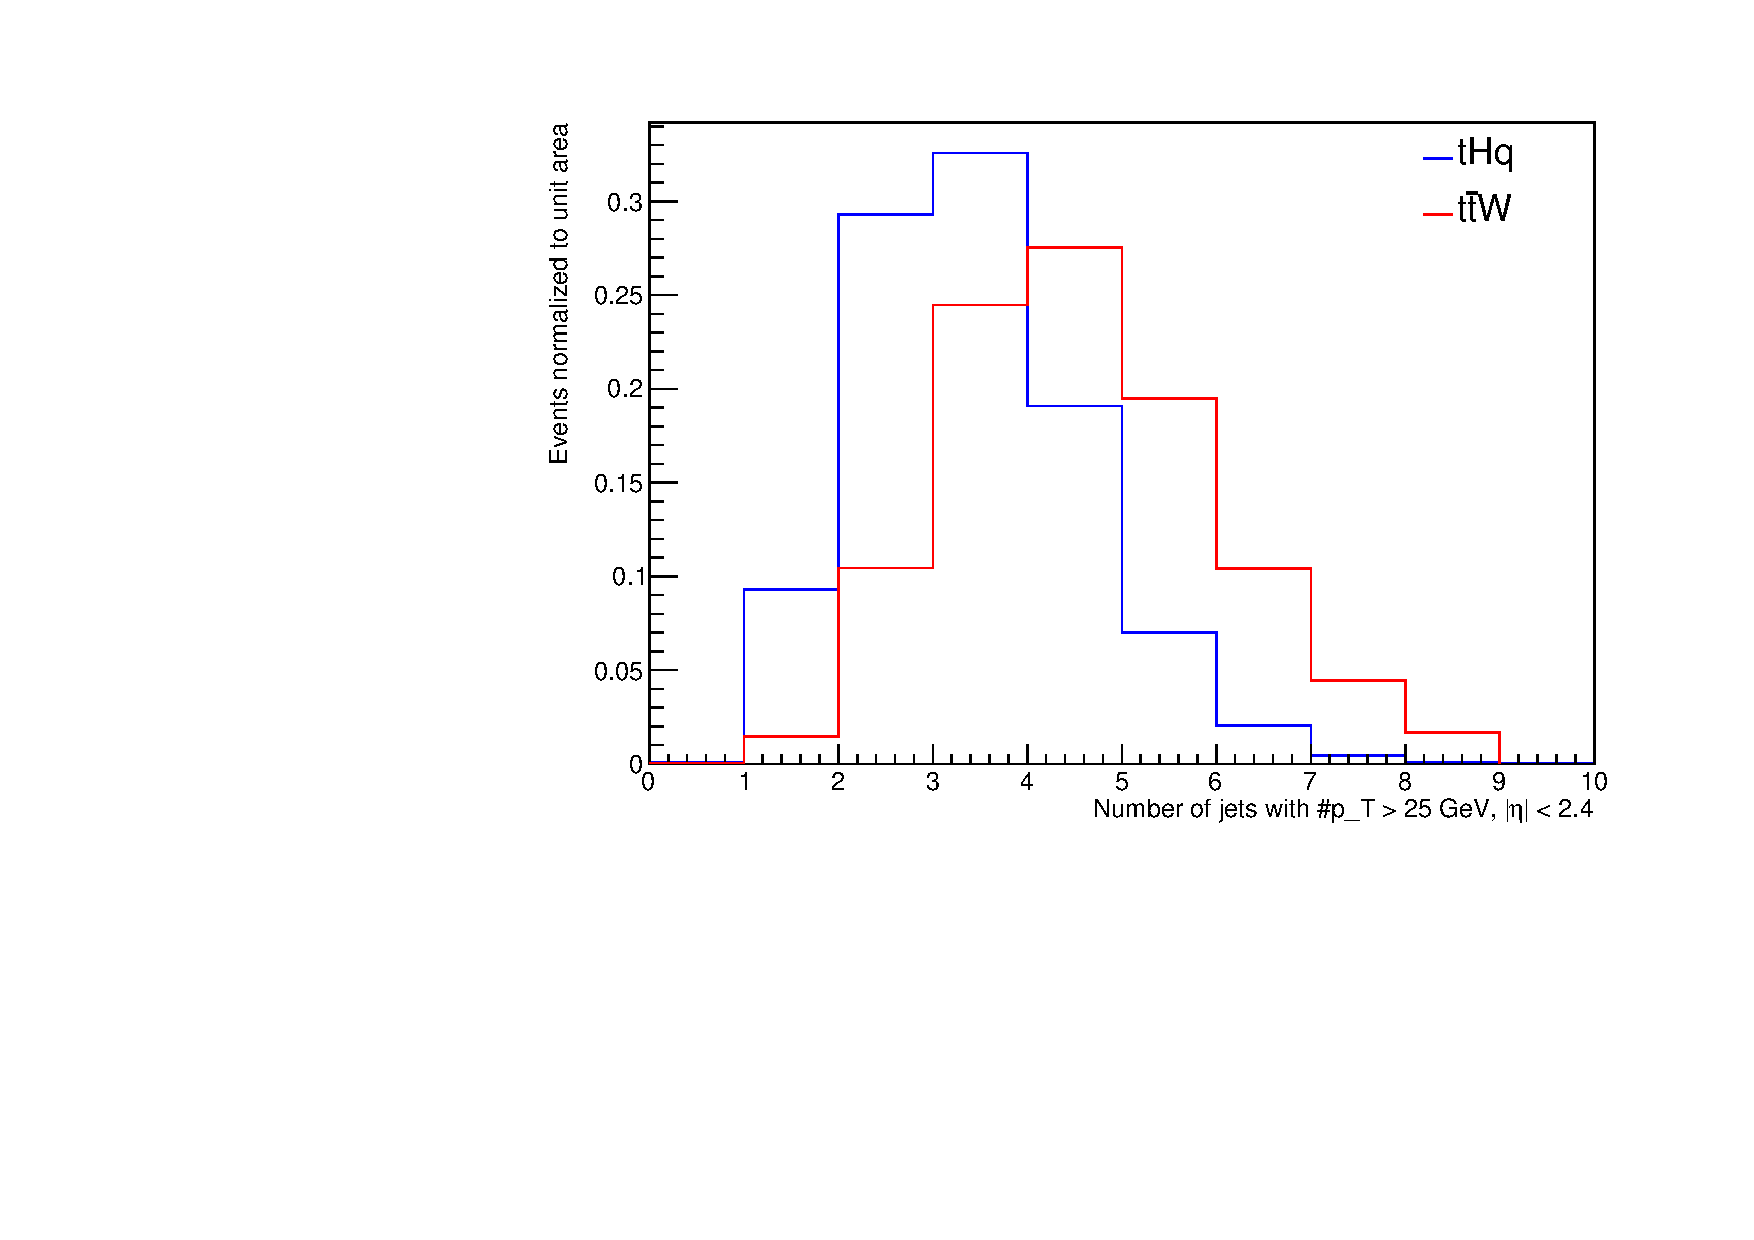
\includegraphics[width=5.5cm,height=3cm]{figures/distributions/compare_variablescompare_variables-ncj24}&
				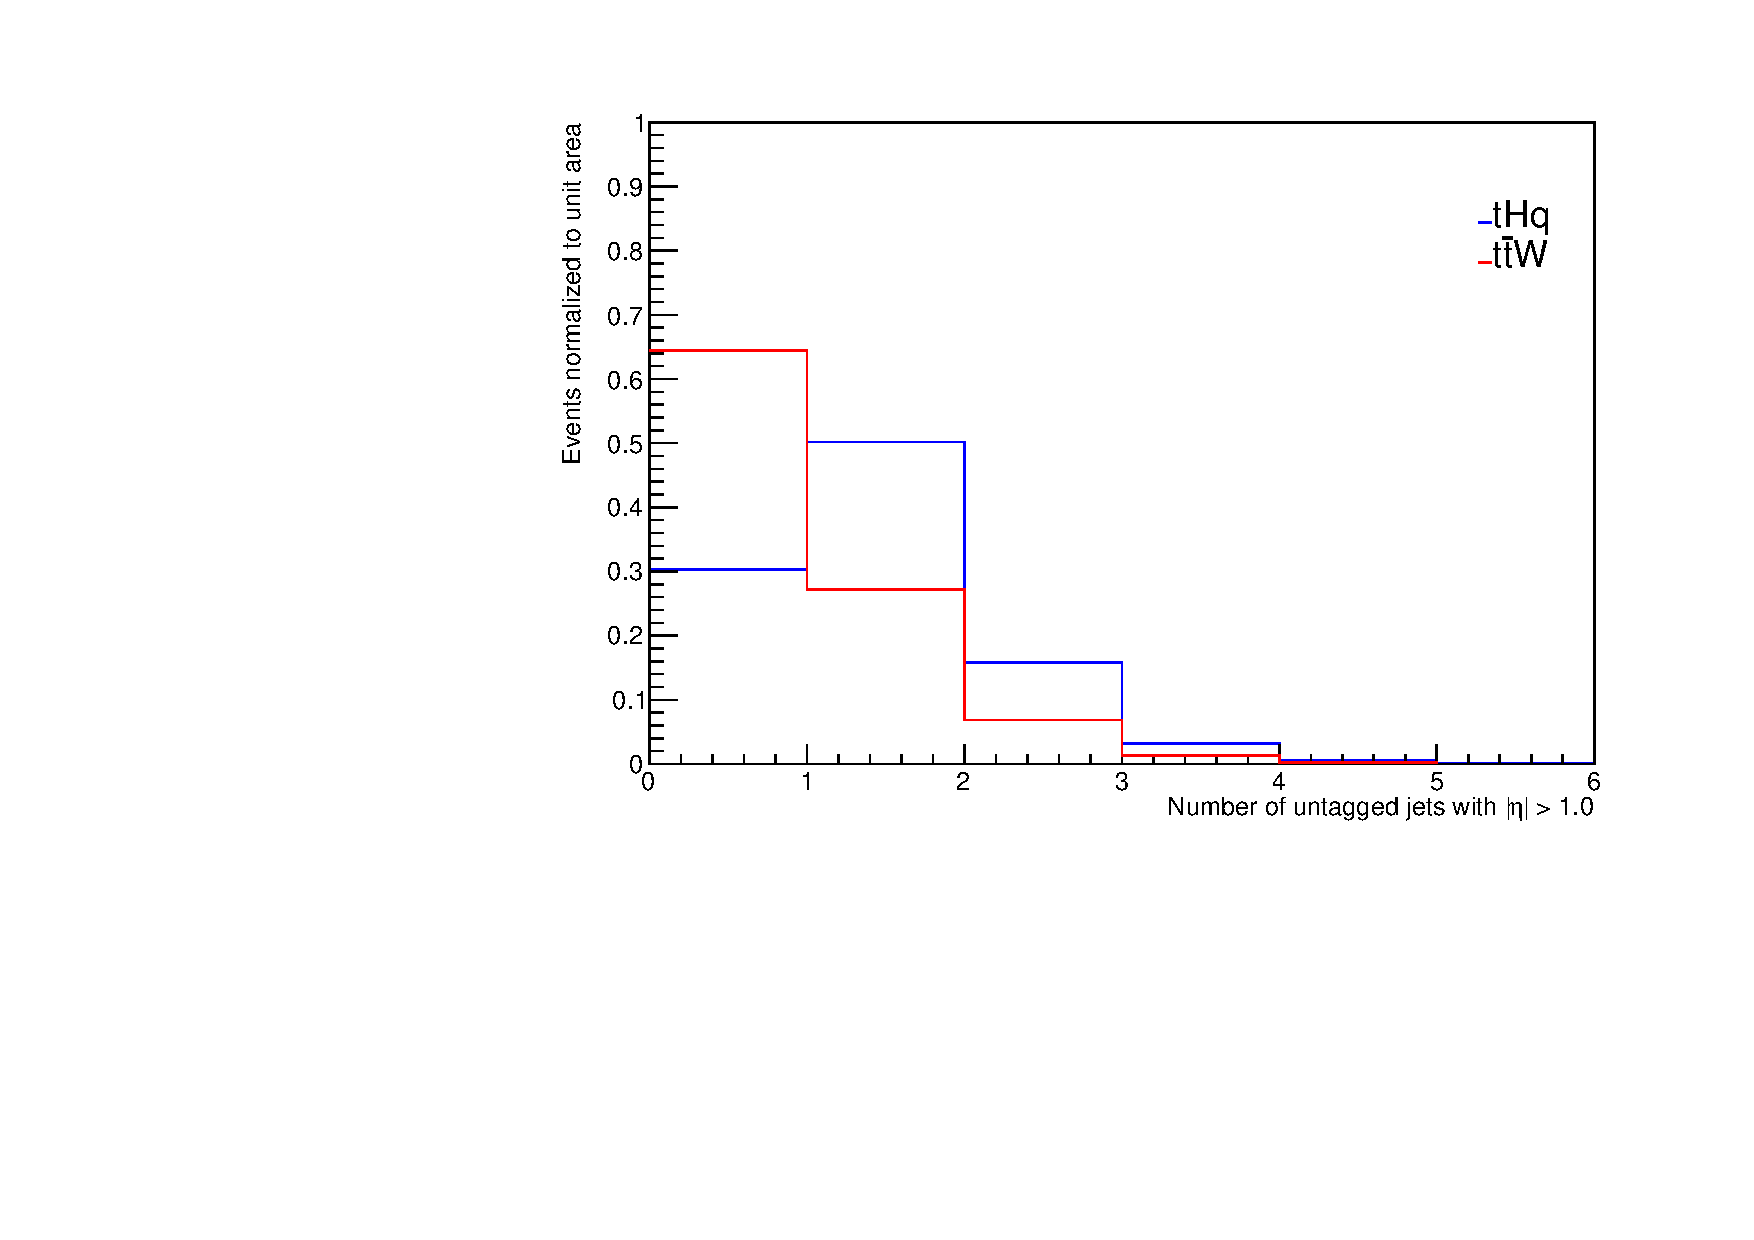
\includegraphics[width=5.5cm,height=3cm]{figures/distributions/compare_variables-nfj}\\		
				{Distribution of selected events with higher pt with a |$\eta$| < 2.4 } & {Distribution of jet events for $|\eta|$>1 } \\
			\end{tabular}
		\end{center}
	\end{frame}
}

{\nologo
	\begin{frame}
		\Fontvi
		\begin{center}
			\begin{tabular}{cc}
				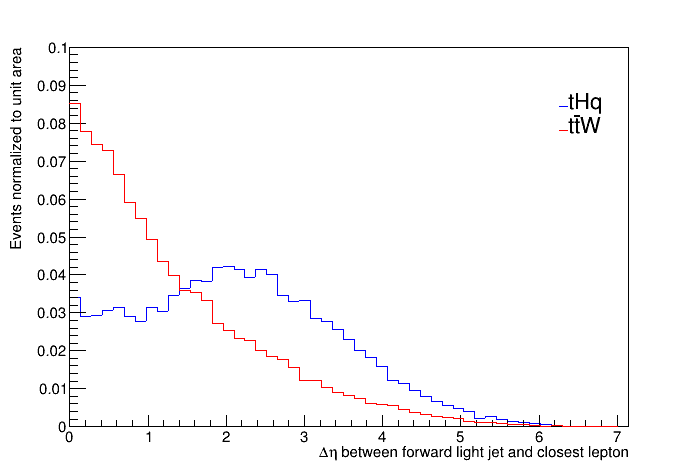
\includegraphics[width=5.5cm,height=3cm]{figures/distributions/compare_variables-eta-fj-cl} &
				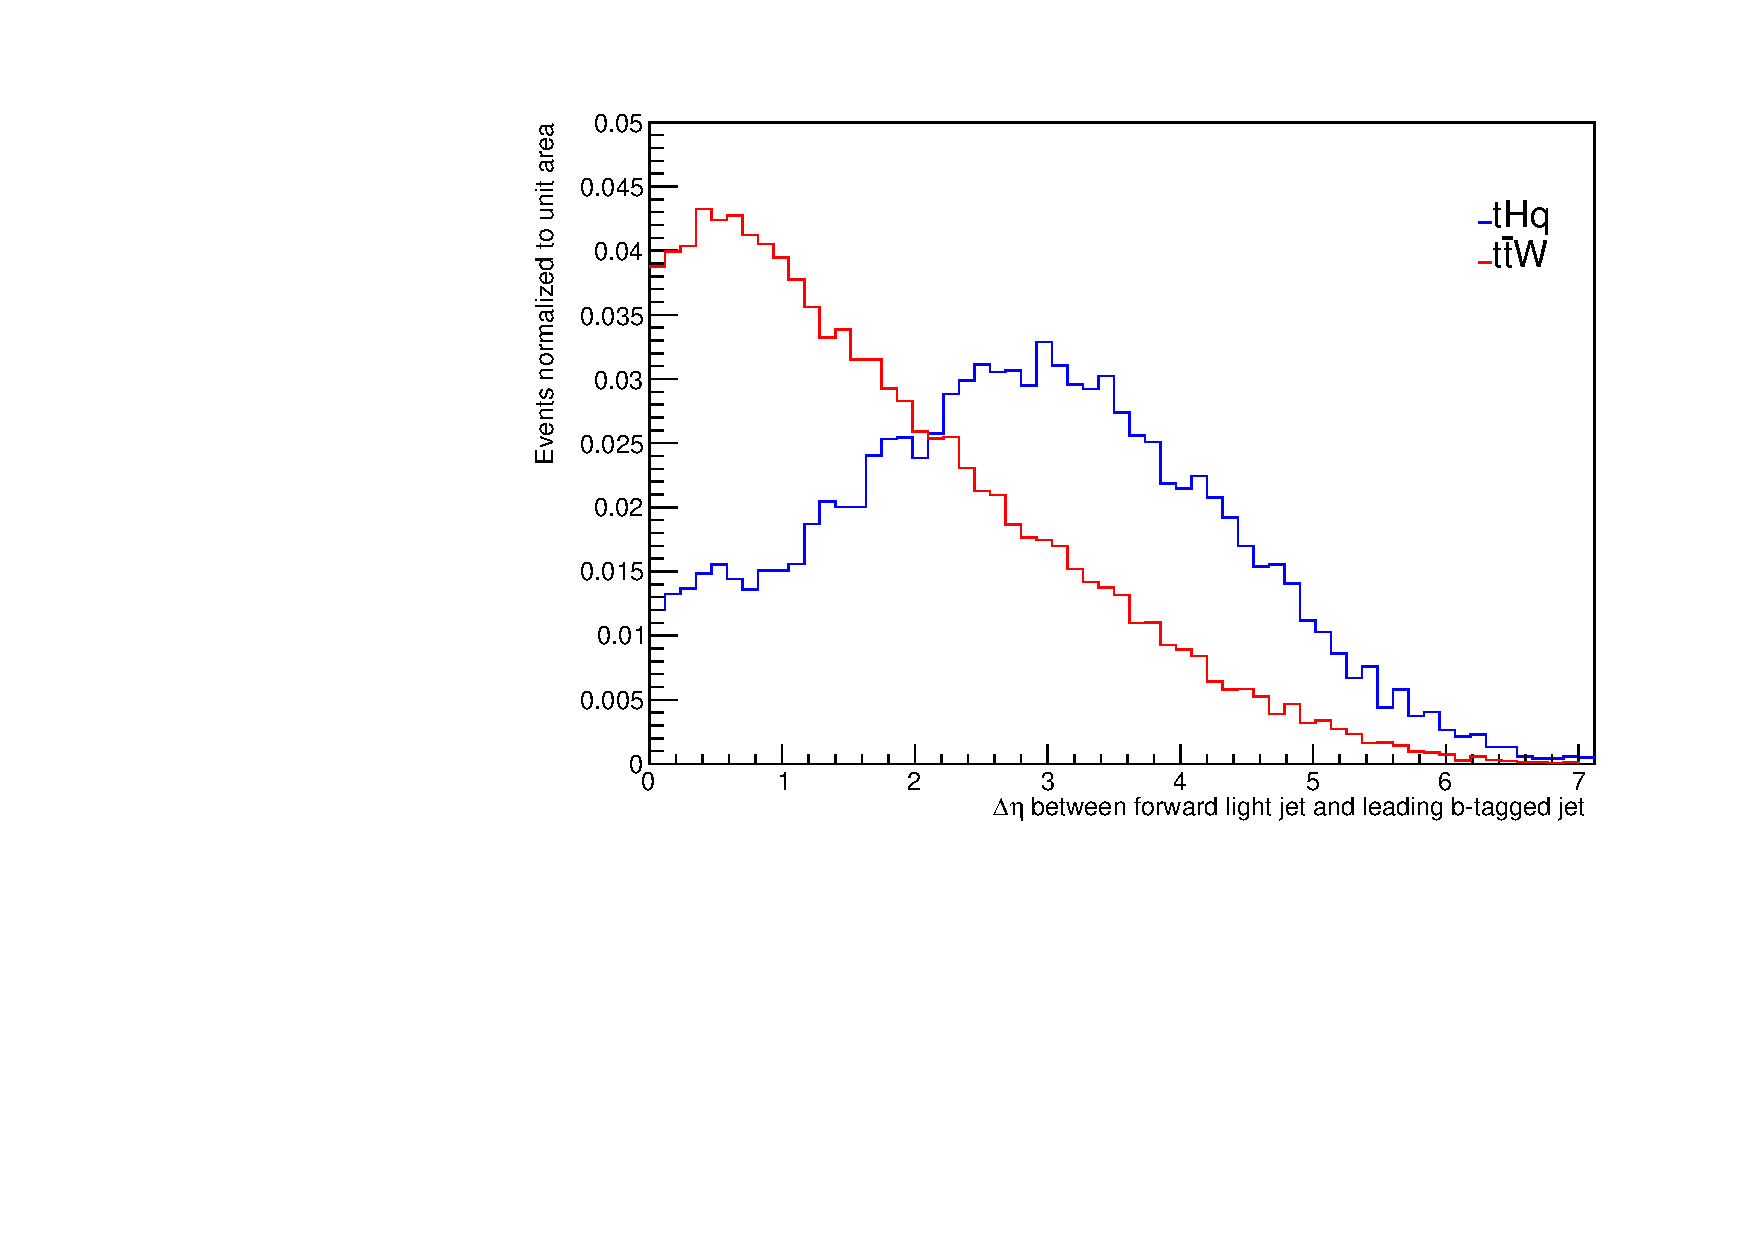
\includegraphics[width=5.5cm,height=3cm]{figures/distributions/compare_variables-eta-fj-b1}\\ 
				{Distribution of events of $|\Delta\eta|$ between a forward jet and the closest lepton} & {	Distribution of events as function of $|\Delta\eta|$ between a forward jet and a b-tagged jet } \\
				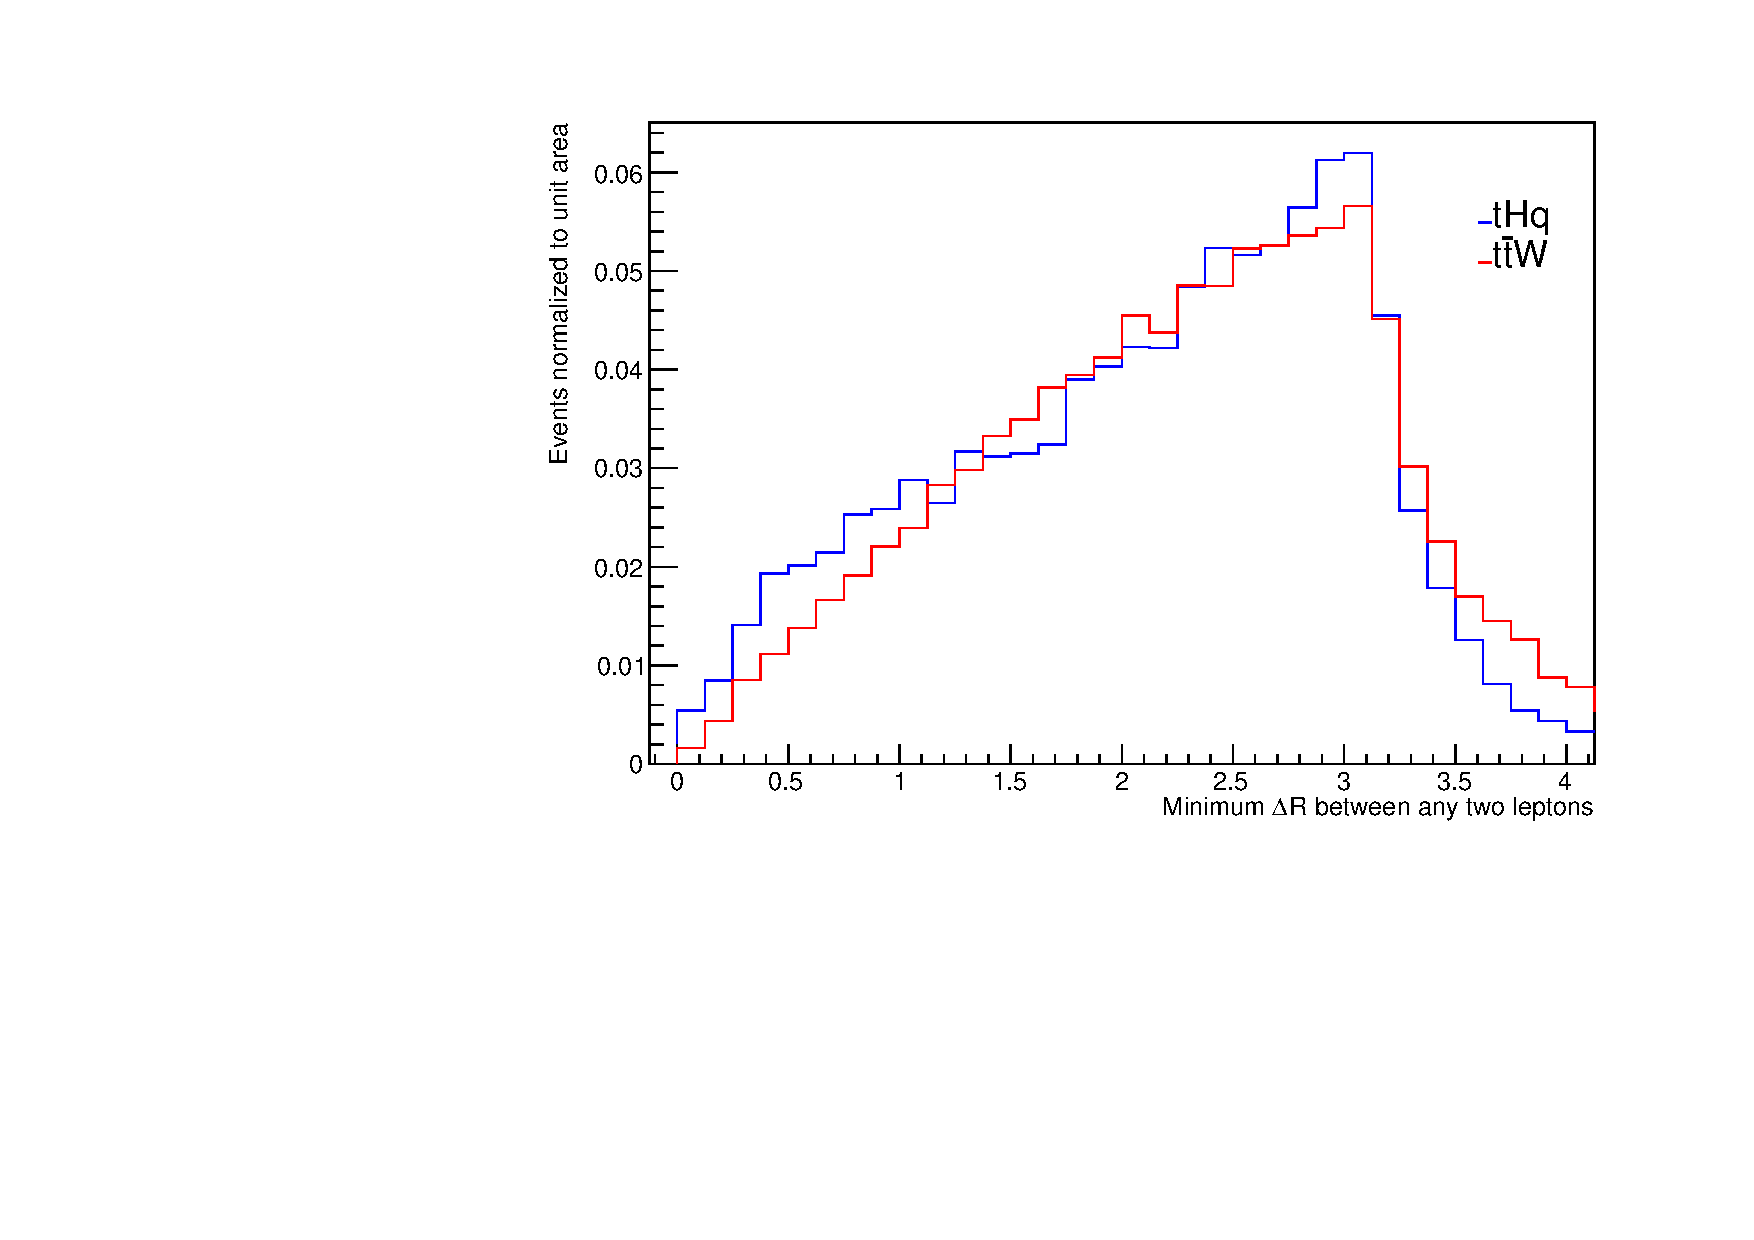
\includegraphics[width=5.5cm,height=3cm]{figures/distributions/compare_variables-dr}&
				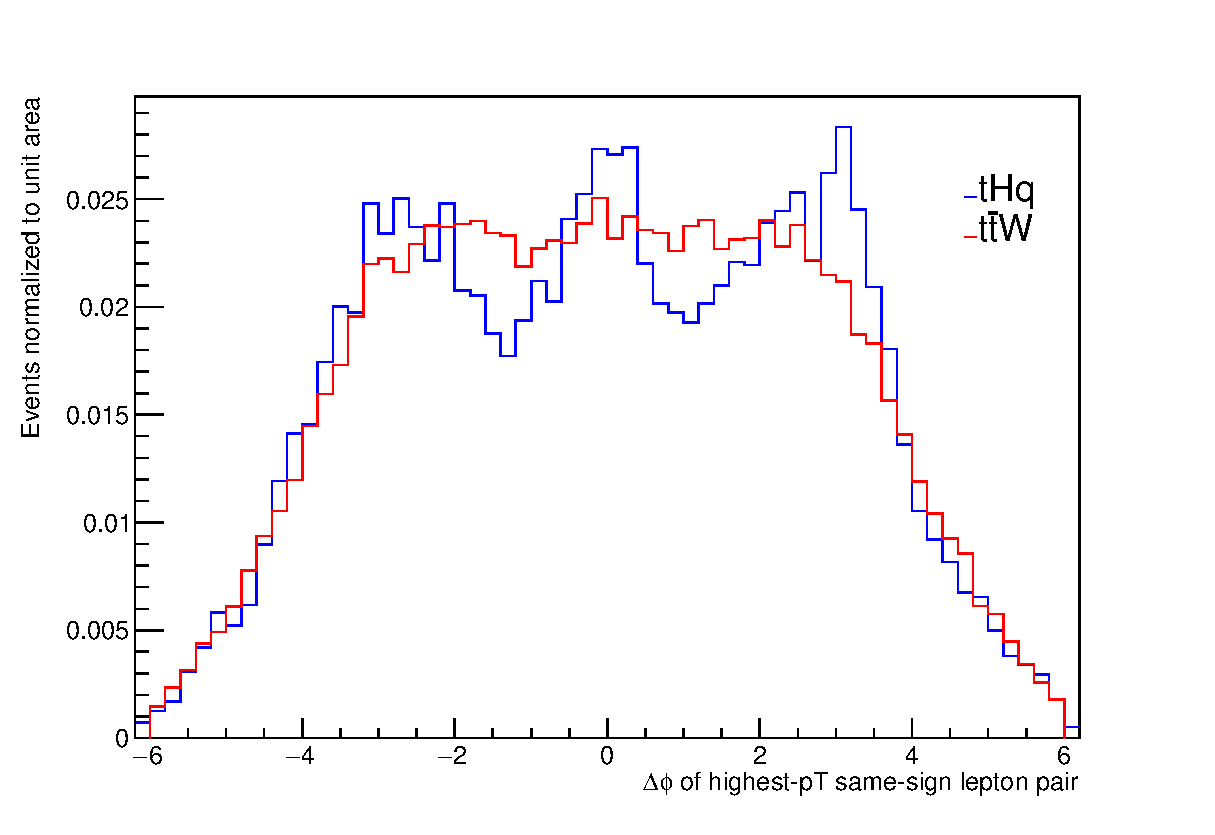
\includegraphics[width=5.5cm,height=3cm]{figures/distributions/compare_variables-phi}\\
				{Distribution of events with a $\Delta R$ between the lepton pairs (highest and lowest pt)} & {Distribution of events of $\Delta\phi$ between the higher pt pair of leptons } \\
			\end{tabular}
		\end{center}
	\end{frame}
}


%\begin{frame}
%\frametitle{Sources of uncertainty on event yields}
%\begin{itemize}
%	\item Luminosity measurement: ~2.6$\%$.
%	\item Data/MC scale factors for lepton selection (ID, iso) and trigger efficiencies ~5$\%$ per lepton.
%	\item Choice of PDF set:
%	\begin{itemize}
%		\item 3.7$\%$ for tHq
%		\item ~4$\%$ for tHW t$\bar{t}$W, t$\bar{t}$Z, t$\bar{t}$H 
%		\item Scale uncertainties: 12$\%$, 4 for t$\bar{t}$W, 10$\%$ for t$\bar{t}$Z, +5.8/-9.2$\%$ for t$\bar{t}$H.
%	\end{itemize}
%	\item Background: WZ, ZZ sample modelling and statistics: ~50$\%$.
%	\item Rare SM (tZ,tri-bosons, WWqq, tttt) : 50$\%$
%	\item Fake rate estimation:
%	The predicted event yield has a normalization uncertainty of ~30-50$\%$ \cite{7}
%\end{itemize}
%\end{frame}




%Closure:  hay jets en los eventos de tt  (gluon-gluon -> tt + gluon ) que se pasan como muones.  jet -> muon =  fake

%Fakes:   proceso de QCD  que genera muchos  jets (por ejemplo  gluon-gluon -> gluons, quarks)  :    jet -> muons  
%fakes are estimated data 

%\footnote[1]{Due to existence of many uncertainties, it is neccesary to sum all the uncertainties. When there is no Correlation, the uncertanties must be summed as the square root of the squares of each uncertainty}



%\begin{frame}
%\frametitle{Sources of systematic uncertainty}
%Detector-simulation related uncertainty
%\begin{itemize}
%\item Calibrations (electron, jet energy scale)
%%\item Efficiencies (particle ID, reconstruction)
%\item Resolutions (jet energy, muon momentum)
%\end{itemize}
%Theoretical uncertainties
%\begin{itemize}
%\item  Factorization/Normalization scale of MC generators
%\item Choice of MC generator (ME and/or PS, e.g. Herwig vs Pythia)
%\end{itemize}
%Monte Carlo Statistical uncertainties
%\begin{itemize}\item Statistical uncertainty of simulated samples\cite{2} \end{itemize}
%\end{frame}

%\begin{frame}
%\begin{figure}
%	\centering
%	
\includegraphics[scale=0.5]{figures/compare_variables}
%	\caption*{Signal and background kinematic distributions}
%\end{figure}
%\end{frame}

%\begin{frame}
%\frametitle{Results}
%\framesubtitle{Likelihood scan}
%\begin{itemize}
%	\item Likelihood function (often simply the likelihood) is a function of the
%	parameters of a statistical model, given specific observed data.
%	\item Likelihood functions play a key role in frequentist inference,
%	especially methods of estimating a parameter from a set of
%	statistics.
%	\item In informal contexts, "likelihood" is often used as a synonym for
%	probability.
%\end{itemize}
%\end{frame}



\end{document}
